% Version 1.2 of SN LaTeX, November 2022
%
% See section 11 of the User Manual for version history 
%
%%%%%%%%%%%%%%%%%%%%%%%%%%%%%%%%%%%%%%%%%%%%%%%%%%%%%%%%%%%%%%%%%%%%%%
%%                                                                 %%
%% Please do not use \input{...} to include other tex files.       %%
%% Submit your LaTeX manuscript as one .tex document.              %%
%%                                                                 %%
%% All additional figures and files should be attached             %%
%% separately and not embedded in the \TeX\ document itself.       %%
%%                                                                 %%
%%%%%%%%%%%%%%%%%%%%%%%%%%%%%%%%%%%%%%%%%%%%%%%%%%%%%%%%%%%%%%%%%%%%%

%%\documentclass[referee,sn-basic]{sn-jnl}% referee option is meant for double line spacing

%%=======================================================%%
%% to print line numbers in the margin use lineno option %%
%%=======================================================%%

%%\documentclass[lineno,sn-basic]{sn-jnl}% Basic Springer Nature Reference Style/Chemistry Reference Style

%%======================================================%%
%% to compile with pdflatex/xelatex use pdflatex option %%
%%======================================================%%

%%\documentclass[pdflatex,sn-basic]{sn-jnl}% Basic Springer Nature Reference Style/Chemistry Reference Style


%%Note: the following reference styles support Namedate and Numbered referencing. By default the style follows the most common style. To switch between the options you can add or remove “Numbered” in the optional parenthesis. 
%%The option is available for: sn-basic.bst, sn-vancouver.bst, sn-chicago.bst, sn-mathphys.bst. %  
 
\documentclass[sn-nature]{sn-jnl}% Style for submissions to Nature Portfolio journals
%%\documentclass[sn-basic]{sn-jnl}% Basic Springer Nature Reference Style/Chemistry Reference Style
%%\documentclass[sn-mathphys,Numbered]{sn-jnl}% Math and Physical Sciences Reference Style
%%\documentclass[sn-aps]{sn-jnl}% American Physical Society (APS) Reference Style
%%\documentclass[sn-vancouver,Numbered]{sn-jnl}% Vancouver Reference Style
%%\documentclass[sn-apa]{sn-jnl}% APA Reference Style 
%%\documentclass[sn-chicago]{sn-jnl}% Chicago-based Humanities Reference Style
%%\documentclass[default]{sn-jnl}% Default
%%\documentclass[default,iicol]{sn-jnl}% Default with double column layout

%%%% Standard Packages
%%<additional latex packages if required can be included here>

\usepackage{graphicx}%
\usepackage{multirow}%
\usepackage{amsmath,amssymb,amsfonts}%
\usepackage{amsthm}%  
\usepackage{mathrsfs}%
\usepackage[title]{appendix}%
\usepackage{xcolor}%
\usepackage{textcomp}%
\usepackage{manyfoot}%
\usepackage{booktabs}%
%\usepackage{algorithm}%
%\usepackage{algorithmicx}%
%\usepackage{algpseudocode}%
\usepackage{listings}%
%%%%
%MAK ADDED

% separate reference sections for the article and the Method
% https://www.overleaf.com/learn/latex/Questions/Creating_multiple_bibliographies_in_the_same_document#The_multibib_package
% \usepackage[sectionbib]{bibunits}
% \defaultbibliographystyle{sn-nature} 
% \defaultbibliography{sn-bibliography}

\newcommand*\degr{\ensuremath{^\circ}}
\newcommand*\arcmin{\ensuremath{^\prime}}
\newcommand*\arcsec{\ensuremath{^{\prime\prime}}}

% for bibliography
\usepackage{natbib}
\def\aap{Astron. \& Astrophys.}
\def\aj{Astron. J.}
\def\apj{Astrophys. J.}
\def\apjs{Astrophys. J. Suppl.}
%\let\apjsupp\apjs
\def\apss{Astrophys. Space Sci.}
\def\araa{Ann. Rev. Astron. Astrophys.}
\def\icarus{Icarus}
\def\mnras{Mon. Not. R. Astron. Soc.}
\def\nat{Nature}
\def\pasp{Proc. Astron. Soc. Pac.}
% Package hyperref Warning: Difference (4) between bookmark levels is greater than one, level fixed on input line 1426.
% 



% \def\apjl{ApJL}
% \def\aj{AJ}
% \def\apj{ApJ}
% \def\pasp{PASP}
% \def\spie{SPIE}
% \def\apjs{ApJS}
% \def\araa{ARAA}
% \def\mnras{MNRAS}
% \def\aap{A\&A}
% \def\nat{Nature}
% \def\icarus{Icarus}






\setcounter{tocdepth}{1}

\newcommand{\asas}{ASASSN-21qj}
\newcommand{\masyr}{mas~yr$^{-1}$}
\newcommand{\teff}{$T_\mathrm{eff}$}
\newcommand{\rsun}{$R_\odot$}

\begin{document}

%TC:ignore

\title[Planetary collision]{A planetary collision afterglow and transit of the resultant debris cloud}

%%=============================================================%%
%% Prefix	-> \pfx{Dr}
%% GivenName	-> \fnm{Joergen W.}
%% Particle	-> \spfx{van der} -> surname prefix
%% FamilyName	-> \sur{Ploeg}
%% Suffix	-> \sfx{IV}
%% NatureName	-> \tanm{Poet Laureate} -> Title after name
%% Degrees	-> \dgr{MSc, PhD}
%% \author*[1,2]{\pfx{Dr} \fnm{Joergen W.} \spfx{van der} \sur{Ploeg} \sfx{IV} \tanm{Poet Laureate} 
%%                 \dgr{MSc, PhD}}\email{iauthor@gmail.com}
%%=============================================================%%


\author[1]{{\fnm{Matthew} \sur{Kenworthy} }\email{kenworthy@strw.leidenuniv.nl}}
\equalcont{These authors contributed equally to this work.}

\author[2]{{\fnm{Simon} \sur{Lock} }\email{s.lock@bristol.ac.uk}}
\equalcont{These authors contributed equally to this work.}

\author[3,4]{{\fnm{Grant} \sur{Kennedy} }\email{G.Kennedy@warwick.ac.uk}}
\equalcont{These authors contributed equally to this work.}

\author[1]{{\fnm{Richelle} \sur{van Capelleveen} }\email{capelleveen@strw.leidenuniv.nl}}
\equalcont{These authors contributed equally to this work.}

\author[5]{{\fnm{Eric} \sur{Mamajek} }\email{Eric.Mamajek@jpl.nasa.gov}}
\equalcont{These authors contributed equally to this work.}

\author[6]{{\fnm{Ludmila} \sur{Carone} }\email{ludmila.carone@oeaw.ac.at}}
\equalcont{These authors contributed equally to this work.}

\author[7,8,9]{{\fnm{Franz-Josef} \sur{Hambsch} }\email{hambsch@telenet.be}}

\author[10]{{\fnm{Joseph} \sur{Masiero} }\email{jmasiero@ipac.caltech.edu}}

\author[11]{{\fnm{Amy} \sur{Mainzer} }\email{amainzer@arizona.edu}}

\author[10]{{\fnm{J. Davy} \sur{Kirkpatrick} }\email{davy@ipac.caltech.edu}}

\author[12,13]{{\fnm{Edward} \sur{Gomez} }\email{egomez@lco.global}}

\author[14]{{\fnm{Zo{\"e}} \sur{Leinhardt} }\email{Zoe.Leinhardt@bristol.ac.uk}}

\author[14]{{\fnm{Jingyao} \sur{Dou} }\email{qb20321@bristol.ac.uk}}

\author[15]{{\fnm{Pavan} \sur{Tanna} }\email{pt426@cam.ac.uk}}

\author[16]{{\fnm{Arttu} \sur{Sainio} }\email{arttu.sainio@elisanet.fi}}

\author[17]{{\fnm{Hamish} \sur{Barker} }\email{hamish.barker@gmail.com}}

\author[18]{{\fnm{St\'{e}phane} \sur{Charbonnel} }\email{stephane.charbonnel@2spot.org}}

\author[18]{{\fnm{Olivier} \sur{Garde} }\email{olivier.garde@2spot.org}}

\author[18]{{\fnm{Pascal} \sur{Le D\^{u}} }\email{pascal.ledu@2spot.org}}

\author[18]{{\fnm{Lionel} \sur{Mulato} }\email{lionel.mulato@2spot.org}}

\author[18]{{\fnm{Thomas} \sur{Petit} }\email{thomas.petit@2spot.org}}

\author[19]{{\fnm{Michael} \sur{Rizzo Smith} }\email{rizzosmith.1@osu.edu}}


\affil[1]{\orgdiv{Leiden Observatory}, \orgname{Leiden University}, \orgaddress{\street{P.O. Box 9513}, \city{Leiden}, \postcode{2300 RA}, \country{The Netherlands}}}

\affil[2]{\orgdiv{School of Earth Sciences}, \orgname{University of Bristol}, \orgaddress{\street{Queens Road}, \city{Bristol}, \postcode{BS8 1QU}, \country{UK}}}

\affil[3]{\orgdiv{Department of Physics}, \orgname{University of Warwick}, \orgaddress{\street{Gibbet Hill Road}, \city{Coventry}, \postcode{CV4 7AL}, \country{UK}}}

\affil[4]{\orgdiv{Centre for Exoplanets}, \orgname{University of Warwick}, \orgaddress{\street{Gibbet Hill Road}, \city{Coventry}, \postcode{CV4 7AL}, \country{UK}}}

\affil[5]{\orgdiv{Jet Propulsion Laboratory}, \orgname{California Institute of Technology}, \orgaddress{\street{4800 Oak Grove Drive}, \city{Pasadena}, \postcode{91109}, \state{CA}, \country{USA}}}

\affil[6]{\orgdiv{Space Research Insitute}, \orgname{Austrian Academy of Sciences}, \orgaddress{\street{Schmiedlstrasse 6}, \city{Graz}, \postcode{A-8042}, \country{Austria}}}

\affil[7]{\orgname{Vereniging Voor Sterrenkunde}, \orgaddress{\street{Oostmeers 122 C}, \city{Bruges}, \postcode{8000 Brugge}, \country{Belgium}}}

\affil[8]{\orgname{American Association of Variable Star Observers}, \orgaddress{\street{185 Alewife Brook Parkway}, \city{Cambridge}, \postcode{MA 02138}, \state{MA}, \country{USA}}}

\affil[9]{\orgname{Bundesdeutsche Arbeitsgemeinschaft f{\"u}r Ver{\"a}nderliche Sterne e. V.}, \orgaddress{\street{Munsterdamm 90}, \city{Berlin}, \postcode{D-12169}, \country{Germany}}}

\affil[10]{\orgdiv{IPAC}, \orgname{Caltech}, \orgaddress{\street{1200 E California Blvd}, \city{Pasadena}, \postcode{MC 100-22}, \state{CA}, \country{USA}}}

\affil[11]{\orgdiv{Lunar and Planetary Laboratory}, \orgname{University of Arizona}, \orgaddress{\street{1629 E. University Blvd.}, \city{Tucson}, \postcode{85721}, \state{AZ}, \country{USA}}}

\affil[12]{\orgdiv{Las Cumbres Observatory}, \orgaddress{\street{6740 Cortona Dr}, \city{Goleta}, \postcode{93117}, \state{CA}, \country{USA}}}

\affil[13]{\orgdiv{School of Physics and Astronomy}, \orgname{Cardiff University}, \orgaddress{\street{The Parade}, \city{Cardiff}, \postcode{CF24 3AA}, \country{UK}}}

\affil[14]{\orgdiv{School of Physics, H H Wills Physics Laboratory}, \orgname{University of Bristol}, \orgaddress{\street{Tyndall Avenue}, \city{Bristol}, \postcode{BS8 1TL}, \country{USA}}}

\affil[15]{\orgdiv{Institute of Astronomy}, \orgname{University of Cambridge}, \orgaddress{\street{Madingley Road}, \city{Cambridge }, \postcode{CB3 0HA}, \country{UK}}}

\affil[16]{\orgname{Independent researcher}, \orgaddress{\street{J{\"a}rvipuistonkatu 7 A 10}, \city{J{\"a}rvenp{\"a}{\"a}}, \postcode{04430}, \country{Finland}}}

\affil[17]{\orgname{Variable Stars South}, \orgaddress{\street{Rutherford Street}, \city{Nelson}, \country{New Zealand}}}

\affil[18]{\orgname{Southern Spectrocopic Project Observatory Team}, \orgaddress{\street{45, Chemin du lac}, \city{Chabons}, \postcode{38690}, \country{FRANCE}}}

\affil[19]{\orgdiv{Department of Astronomy}, \orgname{The Ohio State University}, \orgaddress{\street{140 West 18th Avenue}, \city{Columbus}, \postcode{43210}, \state{OH}, \country{USA}}}





%%==================================%%
%% sample for unstructured abstract %%
%%==================================%%

\abstract{
Planets grow in rotating disks of dust and gas around forming stars, some of which can subsequently collide in giant impacts after the gas component is removed from the disk \cite{Williams11,Wyatt15,Hughes18}.
%
%The remaining solid material forms so-called debris disks which contain planetesimals that, through collisional cascades, generate large amounts of dust that are heated by the star to black body temperatures of 70 to 300\,K \cite{Chen06,Hillenbrand08}.
%
%These are detected as excess infrared emission \cite{Wyatt08,Rieke05,Su06} that decays smoothly with time as the dust is depleted  \cite{2003ApJ...598..626D,Kenyon04,Wyatt08}.
%
%Collisions between planets are a key process in planet formation \citep{Schlichting2018a,DAngelo2018}. 
%
Monitoring programs with the warm Spitzer mission have recorded significant and rapid changes in mid-infrared output for several stars, interpreted as variations in the surface area of warm dusty material ejected by planetary-scale collisions and heated by the central star: e.g., NGC 2354–ID8 \cite{2014Sci...345.1032M,Su19}, HD 166191 \cite{Su22} and V844 Persei \cite{2021ApJ...918...71R}.
%
%However, observational constraints on the aftermath and frequency of such impacts are difficult to obtain.
%
Here we report combined observations of the young ($\sim$~300~Myr), solar-like star \asas{}: an infrared brightening consistent with a blackbody temperature of 1000 K and a luminosity of 4\% of that of the star lasting for about 1000\,days, partially overlapping in time with a complex and deep wavelength-dependent optical eclipse that lasted for about 500 days.
%
The optical eclipse started 2.5\,years after the infrared brightening, implying an orbital period of at least that duration.
%
These observations are consistent with a collision between two exoplanets of several to tens of Earth masses at 2-16\,au from the central star. 
%
Such an impact produces a hot, highly-extended post-impact remnant with sufficient luminosity to explain the infrared observations.
%
Transit of the impact debris, sheared by orbital motion into a long cloud, causes the subsequent complex eclipse of the host star.
%
% Direct observation of a post-impact remnant will revolutionize our understanding of giant impacts, and continued observations will provide new insight into the processes of planet formation.
}



% % █ █▄░█ ▀█▀ █▀█ █▀█ █▀▄ █░█ █▀▀ ▀█▀ █ █▀█ █▄░█
% % █ █░▀█ ░█░ █▀▄ █▄█ █▄▀ █▄█ █▄▄ ░█░ █ █▄█ █░▀█

% Planets grow in rotating disks of dust and gas around forming stars. 
% %
% Towards the end of the planet-forming epoch the majority of the circumstellar gas is removed through accretion on to the star, photoevaporation, and stellar winds \cite{Williams11,Wyatt15,Hughes18}. The solid material that is left behind, ranging from dust to planetary embryos, forms so-called debris disks. These disks are analogues of the Solar system's Asteroid and Edgeworth-Kuiper belts.
% %
% Freed of the damping effects of the gas, collisional cascades break down planetesimals that orbit the star into smaller and smaller debris, until the smallest grains are cleared out of the system by the radiation pressure from the star \cite{Wyatt08}.
% %
% This dust is heated by the star, producing infrared emission with spectral energy distributions described with black body temperatures of 70 to 300\,K \cite{Chen06,Hillenbrand08} and constant fractional luminosities $f = L_{dust}/L_{star}<10^{-3}$ \cite{Wyatt08}.
% %
% The brightness of these disks falls with increasing age, consistent with depletion of material from the birth belts as predicted by theory \cite{2003ApJ...598..626D,Kenyon04,Wyatt08} and agreeing with observational studies \cite{Rieke05,Su06}.
% %
% However, superimposed on this smooth decay are sudden outbursts of flux from large  dust clouds produced by energetic collisions between the largest planetesimals and/or planetary embryos  \cite{2007ApJ...658..569W,2012Natur.487...74M,Meng12,Schneider13}.
% %
% Monitoring programs with the warm Spitzer mission have recorded significant and rapid changes in mid-infrared output consistent with planetary collisions around several stars, e.g., NGC 2354–ID8 \cite{2014Sci...345.1032M,Su19}, HD 166191 \cite{Su22}. 
% %
% These systems are referred to as Extreme Debris Disks \cite[EDDs;][]{Balog09} due to their warmer dust temperatures and significantly higher infrared luminosity compared to a typical debris disk ($f \gtrsim 10^{-2}$).



\keywords{exoplanets, planet formation, debris disks}
%TC:endignore

\maketitle

\section{Main Article}\label{sec1}


% 262 words



% ▀█▀ █░█ █▀▀   █▀▀ █░█ █▀▀ █▄░█ ▀█▀
% ░█░ █▀█ ██▄   ██▄ ▀▄▀ ██▄ █░▀█ ░█░

The otherwise unremarkable star 2MASS J08152329-3859234 underwent a sudden optical dimming event in December 2021 \cite{RizzoSmith21,RizzoSmith22} and was assigned the identifier \asas{} by the ASAS-SN survey \citep{shappee_man_2014,kochanek_all-sky_2017}.
%
Here, we combine both optical (from the Las Cumbres Observatory Global Telescope, LCOGT) and infrared (from the WISE satellite) observations of \asas~for the years before and after this dimming event (Figure~\ref{fig:wisephot}). 
%
Optical multiband photometry shows a wavelength dependent depth consistent with extinction by sub-micron particles.
%
About 900 days prior to the optical dimming event, the \asas~system showed a significant brightening in the infrared, of 0.4 magnitudes at 3.8 microns ($W1$) and 0.8 magnitudes at 4.5 microns ($W2$).
%
Before this time the IR brightness was consistent with being purely stellar.
%
The increased IR fluxes indicate that in addition to the quiescent stellar flux, there was new emission at a temperature of approximately 1000\,K.
%
Such a remarkable combination of observations, particularly the 2.5\,year delay between the IR and optical variation, requires an explanation.

\begin{figure}
\begin{centering}
\includegraphics[width=\textwidth]{all_phot_nature_delta_flux.pdf}
\caption{Optical and infrared photometry of ASASSN-21qj.
%
Panel {\bf a} is normalised optical photometry from ASAS-SN in $V$-band and $g'$ band.
%
Panel {\bf b} shows the fractional flux increase in brightness of ASASSN-21qj in both the $W1$ and $W2$ bands, where a value of 1.0 represents the stellar contribution alone.
%
Panel {\bf c} shows the calculated $NEOWISE$ color temperature estimated from the photometry of the two bands.
%
The color temperature is plotted as zero when there is no IR excess, and is consistent with a temperature of 1000\,K while the excess is present.
%
Error bars are shown at $1\sigma$ confidence.
}
\label{fig:wisephot}
%\script{plot_all_photometry.py}
\end{centering}
\end{figure}


% █ █▀█   █▀▄ █░█ █▀ ▀█▀   █░░ █▀█ █▀▀ ▄▀█ ▀█▀ █ █▀█ █▄░█
% █ █▀▄   █▄▀ █▄█ ▄█ ░█░   █▄▄ █▄█ █▄▄ █▀█ ░█░ █ █▄█ █░▀█

% █▀█ █▀█ ▀█▀ █ █▀▀ ▄▀█ █░░   ▄▀█ █▄░█ █▀▄   █ █▀█   █▀▀ █░█ █▀█ █░█ █▀▀ █▀
% █▄█ █▀▀ ░█░ █ █▄▄ █▀█ █▄▄   █▀█ █░▀█ █▄▀   █ █▀▄   █▄▄ █▄█ █▀▄ ▀▄▀ ██▄ ▄█

The optical and infrared light curves (Figure \ref{fig:wisephot}) provide key constraints on any proposed scenario.
%
The post-brightening IR fluxes in the $W1$ and $W2$ WISE passbands are consistent with emission at a blackbody temperature of $1000 \pm 100$\,K and this temperature is sustained, within error, for the remainder of our observation window, despite a decline in the total flux.
%
For an emitter located at the distance of ASASSN-21qj from Earth, and the observed  maximum luminosity of approximately 0.04\,$L_\star$, this implies an emitting area of 0.01\,au$^2$, equivalent to an object with a radius of 7\,$R_\odot$, or $750$\,$R_{\rm Earth}$.
%
If this emission was from material -- e.g., dust -- passively heated by proximity to the star, then that material must have been generated and remained within about 0.1\,au to produce the observed temperature.

% █▀█ █░░ ▄▀█ █▄░█ █▀▀ ▀█▀   █▀▀ █▀█ █░░ █░░ █ █▀ █ █▀█ █▄░█
% █▀▀ █▄▄ █▀█ █░▀█ ██▄ ░█░   █▄▄ █▄█ █▄▄ █▄▄ █ ▄█ █ █▄█ █░▀█

One possible explanation is that we are observing two unrelated but coincidental phenomena: a warm dust generating collision within 0.1 au of the star, with a separate object transiting the star 900 days later.
%
Two events that are themselves very rare occurring independently in one system is, however, highly improbable.
%
A second explanation is that warm dust is generated close to the star and causes the optical transit, but this requires a fine-tuned configuration where the star is optically blocked by scale height variations in the resulting disk.

Instead, we hypothesize that are we are observing the aftermath of a single collision between super-Earths or mini Neptunes -- a so-called giant impact -- between 2 and 16\,au from the star. 
%
These distances are determined, respectively, by the delay between the IR brightening and the optical eclipse (Fig. \ref{fig:wisephot}), and by gradients in the optical light curve (Fig. \ref{fig:eclipse_overview}).
%
In contrast to other extreme debris disk events where the star heats the dust, we propose that the infrared emission is directly from the post-impact body \cite{Lock2017,2009ApJ...704..770M}, and that impact debris produced the optical transit.
%
Giant impacts are a common occurrence in planet formation \cite{Schlichting2018a,DAngelo2018} and also occur during instabilities in older systems \cite{Kaib2016}; this would explain the observations with a single event of a type that are expected for systems with ages like \asas{}.

Giant impacts are one of the most energetic events planets experience.
%
For example, the kinetic energy of impacts between two half-Neptune-mass bodies range from $10^{33}$ to $10^{34}$~J, enough to vaporize the colliding bodies several times over.
%
A large fraction of this energy is dissipated in the colliding bodies and post-impact bodies are substantially melted and vaporized \cite{Nakajima2015,Lock2017,Carter2020}.
%
Furthermore, extreme torques exerted in impacts often produce rapidly rotating bodies \cite{Lock2017}.
%
Such low density and rotationally-flattened bodies can be hundreds of times larger than the pre-impact planets \cite{Lock2017} with correspondingly large radiative surfaces.

% 205 words

Giant impacts produce significant amounts of debris, typically around 1\% of the colliding mass, that is injected into orbit around the host star\cite{Canup2001,Lock18}.
%
Impact ejecta has a wide range of sizes, from sub-micron dust to planetesimals of tens to hundreds of kilometers, and often contains the most highly heated material \cite{Benz2008_Mercury_book,Leinhardt2015,Carter2020a}.
%
For sufficiently high impact velocities ($>1$~km~s$^{-1}$ for water ice, and $>8$~km~s$^{-1}$ for forsterite) a substantial fraction of this material is vaporised \cite{Stewart2008,Davies2020,Carter2020a}.
%
Shearing of droplets and cooling and condensation of vapor produces a population of small dust grains and solid spherules.
%
The size distribution of this fraction of the debris is uncertain, due to difficulties in modelling condensate nucleation and breakup, but previous work suggests that debris could range in size from sub-micron to decimeters \cite{Benz2008_Mercury_book,Johnson2015}.
%
The wavelength-dependent eclipse suggests that the optical depth of the transiting dust cloud is dominated by sub-micron grains, consistent with these previous estimates.
%
While the fading of the excess infrared flux occurs within 100 days of the start of the optical transit, we consider the timing to be coincidental because there is no clear correspondence between the light curves, for example no  change in the (six month cadence) IR flux when the star dims in the optical wavelengths just before MJD 59500.

% 200 words


\begin{figure*}
\begin{centering}
\includegraphics[width=1.0\textwidth]{master_lightcurve_nature_simple.pdf}
      \caption{The light curve of ASASSN-21qj from several different photometric surveys and the derived transverse velocities.
      %
      Panel {\bf a} shows that the eclipse depth is deeper for shorter wavelengths, indicating that the transiting material is dominated by sub-micron sized grains.
      %
      Panel {\bf b} shows the  transverse velocities derived from the light curve gradients.
      %
      These are lower limits to the true velocity, and thus imply that the transiting material is closer to the star than 16\,au.
      %
      Error bars are shown at $1\sigma$ confidence.
      }
        \label{fig:eclipse_overview}
 %       \script{plot_master_lightcurve.py}
\end{centering}
\end{figure*}



% █▀█ █▀▀ █▀▄▀█ █▄░█ ▄▀█ █▄░█ ▀█▀   █▀ █ ▀█ █▀▀
% █▀▄ ██▄ █░▀░█ █░▀█ █▀█ █░▀█ ░█░   ▄█ █ █▄ ██▄

The radiative flux from post-impact bodies has not been explored in depth.
%
Computational resource limitations make resolving the low-density outer regions and photosphere of post-impact bodies extremely challenging.
%
However, preliminary simulations of impacts between super-Earth and mini-Neptunes place an approximate lower limit on the extent of post-impact bodies and show that post-impact bodies can extend to hundreds of Earth radii.
%
Such an object radiating at $\sim$1000~K would produce a flux comparable to the 0.04~$L_*$ inferred from our observations. 

Independent of impact simulations, there are fundamental limits on the size of post-impact bodies from the Hill and Bondi radii.
%
Any post-impact structure must lie within the Hill sphere, the distance within which the gravity of an object dominates over that of the star.
%
Furthermore, only vapor within the Bondi radius would be bound to the post-impact body.
%
Figure~\ref{fig:Hill_Bondi_R}A shows the Hill radii at different distances from ASASSN-21qj (solid lines) and the Bondi radius for example gas species (dotted lines).
%
Beyond 2.4\,au, the Hill radii of greater than Earth-mass bodies are large enough to accommodate a post-impact body capable of producing the required IR flux ($\sim7R_*$, dotted line). 
%
Heavier gases (H$_2$O, SiO, and SiO$_2$) are also bound to bodies of more than a few Earth masses.
%
A post-impact body of a few Earth masses can hence theoretically produce the observed IR emission, with a photosphere that is dust and/or vapor.


% % 291 words
% \begin{figure}
% \begin{centering}
% \includegraphics[width=\columnwidth]{Hill_Bondi_radii.pdf}
% \caption{A post-impact body of a few to tens of Earth masses could be large enough to explain the observed increase in thermal emission from ASASSN-21qj.
% %
% Shown are the Hill radii for bodies at different semi-major axis (solid colored lines) and the Bondi radii (dotted lines) assuming different compositions for the relevant vapor.
% %
% The horizontal black dashed line shows the radii required to explain the observed flux at the inferred emission temperature of 1000~K. 
% }
% \label{fig:Hill_Bondi_R}
% \end{centering}
% \end{figure}




\begin{figure}
\begin{centering}
\includegraphics[width=\columnwidth]{Size_cooling_combined_figure.pdf}
\caption{The size and temporal evolution of a post-impact body.
%
A post-impact body of a few to tens of Earth masses could be large enough to explain the observed increase in thermal emission from ASASSN-21qj and the subsequent infrared fluxes.
%
Panel {\bf a} shows the Hill radii for bodies at different semi-major axis (solid colored lines) and the Bondi radii (dotted lines) assuming different compositions for the vapor of the post-impact body.
%
The horizontal black dashed line shows the radii required to explain the observed flux at the inferred emission temperature of 1000~K. 
%
The change in excess flux due to a post-impact body with time for a simple model of cooling of a post-impact body for different power-law surface density profiles is in panel {\bf b}, eqn~\ref{eqn:sigma} and for different mass bodies in panel {\bf c}.
%
Each example had an initial radius of 7\,$R_\odot$, a radiative temperature of 1000~K, and a corresponding initial flux of 0.04\,$L_\star$, as estimated for the observed infrared emittor.
%
The solid lines are profiles that can have non-zero initial density at the initial emitting radius, and the dashed lines are for ones that are forced to have zero density at the initial emitting radius.
%
When not stated, the mass of the post-impact body was 50~$M_{\rm Earth}$, the power law exponent is $-2$, and the size of the central region was 10~$R_{\rm Earth}$.
}
\label{fig:Hill_Bondi_R}
\end{centering}
\end{figure}

% █░█░█ ▄▀█ ▀█▀ █▀▀ █▀█   ▄▀█ █▀   █▀▀ █▀█ █▀█ █░░ ▄▀█ █▄░█ ▀█▀
% ▀▄▀▄▀ █▀█ ░█░ ██▄ █▀▄   █▀█ ▄█   █▄▄ █▄█ █▄█ █▄▄ █▀█ █░▀█ ░█░

A key line of evidence for direct detection of a post-impact body is the constant emission temperature.
%
It is argued \cite{Lock18} that rocky post-impact bodies become optically thin at low pressures where radiative loss drives rapid condensation of the rock vapor.
%
The emission temperature is then set by the liquid-vapor phase boundary and is constant until the post-impact body almost fully condenses \cite{Lock18,Caracas2023}.
%
The dew point (onset of condensation) and bubble point (onset of substantial vaporization) of material with bulk silicate Earth composition are similar \cite[$\sim2300$~K, within $\sim 100$~K;][]{Lock18,Fegley2023_BSE_cond} at the low pressures of the photosphere of a post-impact body.
%
%This high temperature is inconsistent with our observations, but the control of emission temperature by the thermodynamics of a material would apply in bodies with different compositions, producing varying radiative temperatures. Specifically, given that we infer the post-impact body to be beyond a few au, water is a likely constituent.
%
%At the low pressures of the photosphere of a post-impact body, water has a vaporization temperature of $\sim250$~K \cite[][]{Wagner2002}, much lower than silicates, but too low to explain the observed $\sim$1000~K emission. 
%
%However, a mixture of water and rock (and potentially other constituents) would have intermediate bubble and dew point temperatures. 
However, even small amounts of water (10$^{-3}$ mole fraction) may lower the bubble and dew points for silicates by $\sim$100~K \cite[][]{Fegley2023_BSE_cond,Lock18}. 
%
The emission temperature of bodies produced by collisions of proto-planets composed of rock and ices/volatiles could be buffered at $\sim$1000~K during early evolution.

% 284 words

% ▀█▀ █ █▀▄▀█ █▀▀   █▀▄ █▀▀ █▀▀ ▄▀█ █▄█
% ░█░ █ █░▀░█ ██▄   █▄▀ ██▄ █▄▄ █▀█ ░█░

The temporal variation of flux from a post-impact body is controlled by evolution of the bodies' size which is governed by a number of competing factors \cite{Lock2018moon,Lock2020}, including radiative energy loss, viscous spreading, and mass and angular momentum transfer by condensates.
%
For silicate-dominated post-impact bodies, the high emission temperature means that radiative cooling dominates, and the post-impact body contracts rapidly, fully condensing over years to thousands of years \cite{Lock2018moon,Lock2020}.
%
The body we observed has a much lower emission temperature, and contracted substantially more slowly.
%
Figure~\ref{fig:Hill_Bondi_R}~B and C show evolution of conceptual post-impact bodies in the limiting case that radiative cooling dominates.
%
If sufficient mass is injected into the outer regions (i.e., less negative power law exponents) the observed flux can remain constant for an initial period and then decays over the order of hundreds of days, in agreement with infrared observations.
%
Further work is required to understand the structure and evolution of bodies produced by impacts between super-Earths and mini-Neptunes of different compositions and identify temporal flux variations consistent with our observations.

% 195 words

% █▀▀ █▀█ █▄░█ █▀▀ █░░ █░█ █▀ █ █▀█ █▄░█ █▀
% █▄▄ █▄█ █░▀█ █▄▄ █▄▄ █▄█ ▄█ █ █▄█ █░▀█ ▄█

% We expect the next decade will result in the detection of several dozen transiting systems similar to \asas, through large scale surveys and triggers provided by ASAS-SN.
% %
% Such observations present an opportunity to study the substructure of debris from planetary collisions, and potentially direct observation of more post-impact bodies.

% Direct observation of a post-impact body would be the first of its kind and offer a valuable insight into key process of planetary system formation  and evolution processes, highly complementary to observations of debris disks and disintegrating planetary material \cite{Gaensike2019,Turner2020,Putirka2021,Blouin2020}.
%
% Furthermore, an impact with enough energy to produce the observed flux could result in the formation of a synestia - a hypothesised class of structures that are likely a common outcome of giant impacts \citep{Lock17}.
%
% Detection of a synestia would transfer a theoretical prediction into a newly-accessible class of planetary object.
%
%It is therefore necessary to obtain rigorous confirmation of any such interpretation of observations.
%
%Possible future observations include IR high contrast imaging to ascertain if the 4-5 microns excess remains a point source, as expected for a post-impact body, or is now extended.
%
%Orbital motion over the next few years will place the post-impact body at about 50 milliarcseconds from the star, marginally resolvable with IR imagers on 8m class telescopes, such as the ERIS camera on the VLT.
%
%In addition, long wavelength spectroscopy could reveal emission or absorption features of silicates or volatiles in the post-impact body.
%
% \asas is a prime target for longer wavelength observations, such as MIRI with the JWST.
%


% , and the substructure of circumplanetary disks that are home to exomoon formation, providing an additional detection and characterisation channel.
%


%\putbib
% 115 words
\clearpage

\setcounter{figure}{0}    

\renewcommand\figurename{Extended Data Fig.}% defined as per springer style 
\renewcommand\tablename{Extended Data Table}%

%\renewcommand\thefigure{Extended \arabic{figure}}    
%\renewcommand\thetable{Extended \arabic{table}}    

%%%%%%%%%%%%%%%%%%%%%%%%%%%  
%%% ███╗░░░███╗███████╗████████╗██╗░░██╗░█████╗░██████╗░░██████╗
%%% ████╗░████║██╔════╝╚══██╔══╝██║░░██║██╔══██╗██╔══██╗██╔════╝
%%% ██╔████╔██║█████╗░░░░░██║░░░███████║██║░░██║██║░░██║╚█████╗░
%%% ██║╚██╔╝██║██╔══╝░░░░░██║░░░██╔══██║██║░░██║██║░░██║░╚═══██╗
%%% ██║░╚═╝░██║███████╗░░░██║░░░██║░░██║╚█████╔╝██████╔╝██████╔╝
%%% ╚═╝░░░░░╚═╝╚══════╝░░░╚═╝░░░╚═╝░░╚═╝░╚════╝░╚═════╝░╚═════╝░
%%%%%%%%%%%%%%%%%%%%%%%%%%%

\section{Methods}\label{sec:methods}

The stellar properties of \asas\ (Gaia DR3 5539970601632026752 = 2MASS~J08152329-3859234) are listed in Extended Data Table~\ref{tab:Stellarprop}, showing that \asas\ is consistent with being a G2 type dwarf star.
%
Where necessary we assume a stellar mass equal to the Sun.
%
\asas\  has a neighbor (Gaia DR3 5539970597334497024 = 2MASS~J08152298-3859244) which is a visual double.
%
Based on the Gaia EDR3 mean ICRS position for epoch 2016.0, the visual companion lies at a separation $\rho$ = $3738.243\pm0.062$ mas and at position angle $\theta$ = $249^{\circ}.977$.
%
Their parallaxes ($\varpi$ = $1.7631\pm0.0112$ mas vs. $1.4711\pm0.0523$ mas) differ by 5.5$\sigma$ and proper motions ($\mu_{\alpha} = -9.692\pm0.012$, $\mu_{\delta} = 7.349\pm0.012$ \masyr\, vs. $\mu_{\alpha} = -0.114\pm0.055$, $\mu_{\delta} = 6.419\pm0.053$ \masyr) differ by a factor of 2.
%
The large differences in distance and proper motions suggests that these stars are not associated.

%\section{Properties of the star}\label{sec:star}


%
% Photometry from various sources was compiled and analysed using the Virtual Observatory SED Analyzer \cite[VOSA; ][]{Bayo08} and the results are listed in Table~\ref{tab:Stellarprop},
%
% GMK response to referee 1 part I and II
% 
The stellar photospheric flux was estimated by fitting stellar models to GAIA, APASS, and DENIS and WISE optical/near-IR photometry (the 2MASS $J$ photometry is an upper limit, and $H$ and $K_s$ are flagged as contaminated).
%
Extended Data Figure \ref{fig:sed} shows the resulting models (the dashed line is discussed below).
%
The ALLWISE photometry ($\sim$2010) is consistent with the NEOWISE photometry pre-brightening nearly ten years later.
%
%The fitting method is outlined by \cite{2019MNRAS.488.3588Y}.

A fit using the method of \cite{2019MNRAS.488.3588Y} with GAIA and DENIS photometry finds that the WISE W1/2 fluxes are about 20\% too high, but better agreement is found with APASS photometry.
%
The difference is explained by the fact that WISE and APASS have lower spatial resolution and include the flux of the $\sim$2\,mag fainter visual double to the West of \asas{} (which is visible in 2MASS).
%
The best fit stellar effective temperature is $5560 \pm 100$\,K.
%
We do not find that reddening is needed for these models; while there is relatively little photometry with which to strongly constrain both $T_{\rm eff}$ and $A_V$, the $T_{\rm eff}$ from GAIA DR3 is $5760 \pm 10$\,K, which suggests that the conclusion of little reddening is valid.
%
Primarily, we conclude that there is no evidence that \asas{} showed evidence for an IR excess before the brightening seen by NEOWISE.

To estimate the IR excess properties we fit the same models, but now including the first five post-brightening NEOWISE data points.
%
We correct for the nearby source by using the GAIA photometry for the star, and the post/pre-brightening difference for the WISE excess flux.
%
This fit yields the fractional luminosity $L_{\rm dust}/L_\star = 0.04 \pm 0.005$ and a dust temperature $950 \pm 30$\,K.
%
To estimate the dust temperature as a function of time we simply subtract the median pre-brightening W1/2 fluxes, with the RMS of these values as the uncertainty (see Figure \ref{fig:wisephot}).
%
The temperature uncertainty increases as the excess fades; the excess flux uncertainty depends on both the observed flux and the stellar flux, and as the excess decreases the stellar uncertainty (which is constant) becomes an increasingly large fraction of the excess.
%
These fluxes therefore exclude the contaminating flux from the nearby object, and are consistent with the SED-derived dust temperature.

Converting dust temperatures to stellocentric radii is uncertain because dust temperature depends on grain size.
%
Typically the radius derived under the assumption of blackbody emission is an underestimate by a factor of up to five \citep{2013MNRAS.428.1263B,2015MNRAS.454.3207P}.
%
Thus, we conclude that the dust location might in the most extreme case be as far as 1\,au, but not sufficiently far to explain the 900\,day delay between the WISE and optical flux variations. which requires a distance of at least 2\,au.


\begin{figure}
    \centering
    \includegraphics[width=0.8\textwidth]{sed.pdf}
    \caption{Spectrum of \asas{}~components. The red symbols show the optical and pre-brightnening WISE IR photometry, and blue symbols show the post-brightnening WISE and ALMA fluxes. Stellar and 1000\,K components consistent with the pre- and post-brightening fluxes are shown. The dashed line shows an estimated cool component spectrum for 0.1\,$\mu$m sized grains associated with the transiting dust cloud. Downward triangles are upper limits.
    %
    Error bars are shown at $1\sigma$ confidence.
}
    \label{fig:sed}
 %   \script{fvsr.py}
\end{figure}
%


\begin{table}
    \centering
    \caption{Properties of \asas}
    \begin{tabular}{@{}lc@{}}
    \hline\hline
Property                               & Value                    \\
        \hline
         $\alpha_{ICRS}$, {[}hh mm ss{]}  & 08:15:23.30\footnotemark[1]  \\
         $\delta_{ICRS}$, {[}dd mm ss{]}  & -38:59:23.3\footnotemark[1]  \\
         $\mu_{\alpha}$ {[}mas yr$^{-1}${]}     & $-9.692\pm0.012$\footnotemark[1]   \\
         $\mu_{\delta}$ {[}mas yr$^{-1}${]}     & $7.349\pm0.012$\footnotemark[1]  \\
         $\varpi$ {[}mas{]}                     & $1.763\pm0.011$\footnotemark[1]   \\
         RV {[}km s$^{-1}${]}                   & $25.8\pm3$\footnotemark[1] \\
         Distance {[}pc{]}                      & $567.2^{+6.7}_{-5.9}$\footnotemark[2] \\ 
        \hline
         $G$ {[}mag{]}                          & $13.371\pm 0.003$\footnotemark[1]  \\
         $G_{BP}$ {[}mag{]}                     & $13.697\pm 0.003$\footnotemark[1]    \\
         $G_{RP}$ {[}mag{]}                     & $12.882\pm 0.004$\footnotemark[1]   \\
         $G_{BP}-G_{RP}$ {[}mag{]}              & $0.815\pm 0.005$\footnotemark[1]         \\
         $J$ {[}mag{]}                          & $>12.07$\footnotemark[3]   \\
         $H$ {[}mag{]}                          & $12.03\pm0.04$\footnotemark[3]    \\
         $K_s$ {[}mag{]}                          & $11.99\pm0.04$\footnotemark[3]    \\
         $B$ (AB) {[}mag{]}                     & $14.16\pm0.06$\footnotemark[4]     \\
         $V$ (AB) {[}mag{]}                     & $13.48\pm0.03$\footnotemark[4]   \\
         $g'$ (AB) {[}mag{]}                     & $13.77\pm0.03$\footnotemark[4]  \\
         $r'$ (AB) {[}mag{]}                     & $13.29\pm0.03$\footnotemark[4]     \\
         $i'$ (AB) {[}mag{]}                     & $13.20\pm0.08$\footnotemark[4]   \\
        \hline
%         $M_*$ [$M_{\odot}$]                    & $0.85\pm0.02$  \\
         \teff{} [K]                            & $5760\pm10$\footnotemark[1]  \\
         {[}Fe/H{]} [dex]                       & $-0.23\pm0.01$\footnotemark[1] \\
         log\,$g$ [log$_{10}$ cm\,s$^{-2}$]     & $4.339\pm0.005$\footnotemark[1]  \\
         $R_*$ [\rsun{}]                        & $1.04$\footnotemark[5] \\
         log($L_{bol}/L_{\odot}$) [dex]         & $0.033$\footnotemark[5] \\
         $m_{bol}$ [mag]                        & $13.49\pm0.02$\footnotemark[6] \\
         $E(G_{BP}-G_{RP})$ {[}mag{]}           & $0.01 \pm 0.005$\footnotemark[6]    \\
         Age [Myr]                              & $300\pm92$\footnotemark[7] \\
         
        \hline
    \end{tabular}
    \footnotetext[1]{Gaia EDR3 \cite{Brown21}, coordinates are J2000 at epoch 2000.0.}
    \footnotetext[2]{\cite{BailerJones21}}
    \footnotetext[3]{2MASS \cite{Cutri03}, $J$ is an upper limit and $H$ and $K_s$ are flagged as contaminated.}
    \footnotetext[4]{APASS \cite{2015AAS...22533616H}, this photometry includes a nearby star.}
    \footnotetext[5]{Estimated from an SED fit fixed to Gaia properties.}
    \footnotetext[6]{Estimated using mean stellar properties \cite{2013ApJS..208....9P}.}
    \footnotetext[7]{Estimated using rotation period.}

\label{tab:Stellarprop}
\end{table}

\subsection*{Observations}\label{sec:obs}

The beginning of the eclipse was announced \cite{RizzoSmith21} by the ASAS-SN survey, which triggered several observing campaigns at optical wavelengths and an ALMA observation at Band 7 (program \texttt{2019.A.00040.S}).
%
The photometric data and passband filters are listed in Extended Data Table~\ref{tab:photometry}.
%



\begin{table}
    \centering
    \caption{Photometric observations of ASASSN-21qj. The number of points are listed per survey and filter. %
    %
    This is the count after initial rejection of photometric points with significantly large error bars.
    %
    Further photometric points may have been rejected in the differeny analysis steps.
    %
    The ROAD observations constitute the majority of observations from the AAVSO data sets.}
    \begin{tabular}{@{}lcc@{}}
    \hline\hline
Survey name  & Filter & Number of points                    \\
        \hline
ASASSN   &  $V$   & 758 \\
   &  $g'$   & 3225 \\
        \hline
ATLAS & $c$ & 161 \\
 & $o$ & 677 \\
        \hline
AAVSO   &  $B$   & 729 \\    % 601 in RVC
   &  $I$   & 728 \\    % 612 in RVC
   &  $V$   & 722 \\    % 599 in RVC
        \hline
LCOGT   &  $g$   & 275 \\    % RVC
   &  $r$   & 224 \\    % RVC
   &  $i$   & 168 \\    % RVC
        \hline
NEOWISE & $W1$ & 18 \\
 & $W2$ & 18 \\
        \hline
    \end{tabular}
 
\label{tab:photometry}
\end{table}

% ░█████╗░░██████╗░█████╗░░██████╗
% ██╔══██╗██╔════╝██╔══██╗██╔════╝
% ███████║╚█████╗░███████║╚█████╗░
% ██╔══██║░╚═══██╗██╔══██║░╚═══██╗
% ██║░░██║██████╔╝██║░░██║██████╔╝
% ╚═╝░░╚═╝╚═════╝░╚═╝░░╚═╝╚═════╝░
%
% 230 words
%
The All Sky Automated Survey \cite[ASAS; ][]{pojmanski_all_1997, asas_2005, asas_2018} is a survey consisting of two observing stations - one in Las Campanas, Chile and the other on Maui, Hawaii. 
%
Each observatory is equipped with two CCD cameras using V and I filters and commercial f $ = 200$ mm, D $= 100$ mm lenses, although both larger (D $=250$ mm) and smaller (50-72 mm) lenses were used at earlier times.
%
The majority of the data are taken with a pixel scale of $\approx$ 15\arcsec{}.
%
ASAS splits the sky into 709 partially overlapping 9\degr{} $\times$ 9\degr{} fields, taking on average 150 3-minute exposures per night, leading to a variable cadence of 0-2 frames per night.
%
Depending on the equipment used and the mode of operation, the ASAS limiting magnitude varied between 13.5 and 15.5 mag in V, and the saturation limit was 5.5 to 7.5 mag. 
%
Precision is around 0.01-0.02 mag for bright stars and below 0.3 mag for the fainter ones. 
%
ASAS photometry is calibrated against the Tycho catalog, and its accuracy is limited to 0.05 mag for bright, non-blended stars.

% ░█████╗░░██████╗░█████╗░░██████╗░░░░░░░██████╗███╗░░██╗
% ██╔══██╗██╔════╝██╔══██╗██╔════╝░░░░░░██╔════╝████╗░██║
% ███████║╚█████╗░███████║╚█████╗░█████╗╚█████╗░██╔██╗██║
% ██╔══██║░╚═══██╗██╔══██║░╚═══██╗╚════╝░╚═══██╗██║╚████║
% ██║░░██║██████╔╝██║░░██║██████╔╝░░░░░░██████╔╝██║░╚███║
% ╚═╝░░╚═╝╚═════╝░╚═╝░░╚═╝╚═════╝░░░░░░░╚═════╝░╚═╝░░╚══╝

The All Sky Automated Survey for Supernovae \cite[ASAS-SN; ][]{shappee_man_2014,kochanek_all-sky_2017} consists of five stations around the globe, with each station hosting four telescopes with a shared mount.
%
The telescopes consist of a 14-cm aperture telephoto lens with a field of view of approximately 4.5\degr{}$\times$4.5\degr{} and an 8.0\arcsec{} pixel scale.
% 
Two of the original stations (one in Hawaii and one in Chile) were initially fitted with $V$ band filters, but now these and all the other stations (Texas, South Africa and a second in Chile) observe with $g'$ band filters down to 18 mag.


% ██████╗░░█████╗░░█████╗░██████╗░
% ██╔══██╗██╔══██╗██╔══██╗██╔══██╗
% ██████╔╝██║░░██║███████║██║░░██║
% ██╔══██╗██║░░██║██╔══██║██║░░██║
% ██║░░██║╚█████╔╝██║░░██║██████╔╝
% ╚═╝░░╚═╝░╚════╝░╚═╝░░╚═╝╚═════╝░

The Remote Observatory Atacama Desert \cite[ROAD; ][]{Hambsch12} is a fully automated telescope located in Chile that obtains nightly photometry in Astrodon B, V and I bands for a wide range of astronomical projects.
%
It consists of a 40-cm $f/6.8$ Optimized Dall-Kirkham and uses a Finger Lakes Instruments camera with a 4k$\times$4k array with pixels of $9\mu m$ in size.
%
Data are reduced using a custom pipeline and then published on the AAVSO website.

% ██╗░░░░░░█████╗░░█████╗░░██████╗░████████╗
% ██║░░░░░██╔══██╗██╔══██╗██╔════╝░╚══██╔══╝
% ██║░░░░░██║░░╚═╝██║░░██║██║░░██╗░░░░██║░░░
% ██║░░░░░██║░░██╗██║░░██║██║░░╚██╗░░░██║░░░
% ███████╗╚█████╔╝╚█████╔╝╚██████╔╝░░░██║░░░
% ╚══════╝░╚════╝░░╚════╝░░╚═════╝░░░░╚═╝░░░

Las Cumbres Observatory Global Telescope (LCOGT) is a network of 25 fully robotic operated telescopes distributed over 7 sites located all around the globe.
%
These telescopes are designed to observe transient astronomical events at optical and near-infrared wavelengths.
%
LCOGT provides a large variety of filter options, but the data we collected are in SDSS $g'$, $r'$ and $i'$ bands.
%
All data is automatically processed and calibrated by the BANZAI pipeline.
%
The visual companion caused complications in BANZAIs automatic aperture extraction routine; sometimes correct apertures were extracted for both \asas\ and the nearby star, and sometimes both sources were extracted in one large aperture, often with an offset from the true center of \asas.
%
%Although the companion is faint, this caused the resulting photometry to be in inaccurate and therefore unusable.
%
To correct this, the last two stages of the BANZAI routine, aperture extraction and photometry calibration, were modified for this specific situation. 
%
The calibrated magnitudes of all sources in the frames are computed using the default BANZAI photometry calibration routine.

% ░█████╗░████████╗██╗░░░░░░█████╗░░██████╗
% ██╔══██╗╚══██╔══╝██║░░░░░██╔══██╗██╔════╝
% ███████║░░░██║░░░██║░░░░░███████║╚█████╗░
% ██╔══██║░░░██║░░░██║░░░░░██╔══██║░╚═══██╗
% ██║░░██║░░░██║░░░███████╗██║░░██║██████╔╝
% ╚═╝░░╚═╝░░░╚═╝░░░╚══════╝╚═╝░░╚═╝╚═════╝░

ATLAS is a project that searches for near earth asteroids down to a magnitude of 19 \cite{Tonry18}.
%
Two filters were obtained, the $o$ (orange) and $c$ (cyan) filters respectively.
%
The data consists of two to four photometric points observed each night when conditions permitted.
%
Photometry with large errors was rejected in a first pass, then the remaining observations during a night were averaged and an error based on the r.m.s. of these nightly points was calculated.
%
The photometry covers the time period where the collision event occurred. 

% ██████╗░░██████╗██████╗░░█████╗░████████╗
% ╚════██╗██╔════╝██╔══██╗██╔══██╗╚══██╔══╝
% ░░███╔═╝╚█████╗░██████╔╝██║░░██║░░░██║░░░
% ██╔══╝░░░╚═══██╗██╔═══╝░██║░░██║░░░██║░░░
% ███████╗██████╔╝██║░░░░░╚█████╔╝░░░██║░░░
% ╚══════╝╚═════╝░╚═╝░░░░░░╚════╝░░░░╚═╝░░░

% A spectrum of the star was taken on 59829.8785 MJD (2022-09-07 at 08:34:52 UT) from the Deep Sky Chile
% %\footnote{\url{https://www.deepskychile.com/en/}}
% site in Chile (at longitude: $70^o 51\arcmin 11\arcsec 86$
% latitude: $30^o S 31\arcmin 34\arcsec 71$ altitude:1700m AMSL).
% %
% The telescope is a Ritchey-Chretien telescope ($d=305$mm) at $f/5$ (with focal reducer CCD 67 astrophysics) on an equatorial mount GM 3000 HPS.
% %from 10 micron\footnote{\url{https://www.10micron.com/en/product/gm3000-hps/}}.
% %
% The spectrograph is a Spectrograph Alpy 600 $R=570$ with a $23\mu m$ wide slit
% % \footnote{\url{https://www.shelyak.com/produit/alpy-600/?lang=en}}
% %
% and an ATIK 414ex camera. %\footnote{\url{https://www.atik-cameras.com/product/atik-414ex/}}.
% %
% The spectrum is composed of three unbinned exposures of 1200s each, taken in automatic mode with Prism V11 Software. %\footnote{\url{https://www.prism-astro.com/}}, and the spectrum is processed with ISIS software\footnote{\url{http://www.astrosurf.com/buil/isis-software.html}}.
% %
%The final spectrum is shown in Figure~\ref{fig:2spotspectrum}.

%The spectrum shows the absorption features of a typical early G-type star, and we see no signs of gas absorption in this spectrum, implying that there is only dust in the intervening material.

% \begin{figure}
%     \begin{centering}
%         \includegraphics[width=0.9\textwidth]{2spot_spectrum.pdf}
% \caption{Continuum normalised spectrum of \asas{}. The main absorption lines are marked with the transition and wavelength.}
%         \label{fig:2spotspectrum}
%         %\script{plot_2spot_spectrum.py}
%     \end{centering}
% \end{figure}



%\section{Analysis}\label{sec:dustcloud}

% ██████╗░░█████╗░████████╗░█████╗░████████╗██╗░█████╗░███╗░░██╗░█████╗░██╗░░░░░
% ██╔══██╗██╔══██╗╚══██╔══╝██╔══██╗╚══██╔══╝██║██╔══██╗████╗░██║██╔══██╗██║░░░░░
% ██████╔╝██║░░██║░░░██║░░░███████║░░░██║░░░██║██║░░██║██╔██╗██║███████║██║░░░░░
% ██╔══██╗██║░░██║░░░██║░░░██╔══██║░░░██║░░░██║██║░░██║██║╚████║██╔══██║██║░░░░░
% ██║░░██║╚█████╔╝░░░██║░░░██║░░██║░░░██║░░░██║╚█████╔╝██║░╚███║██║░░██║███████╗
% ╚═╝░░╚═╝░╚════╝░░░░╚═╝░░░╚═╝░░╚═╝░░░╚═╝░░░╚═╝░╚════╝░╚═╝░░╚══╝╚═╝░░╚═╝╚══════╝

% ██████╗░███████╗██████╗░██╗░█████╗░██████╗░
% ██╔══██╗██╔════╝██╔══██╗██║██╔══██╗██╔══██╗
% ██████╔╝█████╗░░██████╔╝██║██║░░██║██║░░██║
% ██╔═══╝░██╔══╝░░██╔══██╗██║██║░░██║██║░░██║
% ██║░░░░░███████╗██║░░██║██║╚█████╔╝██████╔╝
% ╚═╝░░░░░╚══════╝╚═╝░░╚═╝╚═╝░╚════╝░╚═════╝░


% ████████╗███████╗░██████╗░██████╗
% ╚══██╔══╝██╔════╝██╔════╝██╔════╝
% ░░░██║░░░█████╗░░╚█████╗░╚█████╗░
% ░░░██║░░░██╔══╝░░░╚═══██╗░╚═══██╗
% ░░░██║░░░███████╗██████╔╝██████╔╝
% ░░░╚═╝░░░╚══════╝╚═════╝░╚═════╝░

The Transiting Exoplanet Survey Satellite \cite[TESS; ][]{2015JATIS...1a4003R} is a satellite designed to survey for transiting exoplanets among the brightest and nearest stars over most of the sky.
%
The TESS satellite orbits the Earth every 13.7 days on a highly elliptical orbit, scanning a sector of the sky spanning 24\degr $\times$ 96\degr\ for a total of two orbits, before moving on to the next sector. 
%
It captures images at a 2 second (used for guiding), 20 seconds (for 1000 bright asteroseismology targets), 120 seconds (for 200 000 stars that are likely planet hosts) and 30 minute (full frame image) cadences.
%
The instrument consists of 4 CCDs each with a field of view of 24\degr$\times$24\degr, with a wide band-pass filter from 600-1000 nm (similar to the $I_C$ band) and provides high precision ($\approx$milli-mag) light curves for stars down to about 14\,mag ($I_C$).
%

% 150 words


% ███╗░░██╗███████╗░█████╗░░██╗░░░░░░░██╗██╗░██████╗███████╗
% ████╗░██║██╔════╝██╔══██╗░██║░░██╗░░██║██║██╔════╝██╔════╝
% ██╔██╗██║█████╗░░██║░░██║░╚██╗████╗██╔╝██║╚█████╗░█████╗░░
% ██║╚████║██╔══╝░░██║░░██║░░████╔═████║░██║░╚═══██╗██╔══╝░░
% ██║░╚███║███████╗╚█████╔╝░░╚██╔╝░╚██╔╝░██║██████╔╝███████╗
% ╚═╝░░╚══╝╚══════╝░╚════╝░░░░╚═╝░░░╚═╝░░╚═╝╚═════╝░╚══════╝

The Near-Earth Object Wide-field Infrared Survey Explorer (NEOWISE) is a space-based infrared telescope that has been surveying the sky since 2013 at $3.4$ and $4.6~\mu$m.
%
NEOWISE orbits near the Earth's day-night terminator, scanning rings of the sky near $\sim90^\circ$ Solar elongation, and obtains a sequence of observations of a given region of sky every six months.
%
The two wavelength channels are obtained simultaneously through a beamsplitter, allowing for color information to be extracted for each source detected in both bands.
%
Detailed descriptions of NEOWISE operations and early results from the Reactivation mission \cite{mainzer14neowise} and the standard data processing and data characteristics \cite{cutri15} are available.
%
A single data point for each epoch and wavelength is calculated by taking the weighted average of the individual NEOWISE measurements.

% ░█████╗░██╗░░░░░███╗░░░███╗░█████╗░
% ██╔══██╗██║░░░░░████╗░████║██╔══██╗
% ███████║██║░░░░░██╔████╔██║███████║
% ██╔══██║██║░░░░░██║╚██╔╝██║██╔══██║
% ██║░░██║███████╗██║░╚═╝░██║██║░░██║
% ╚═╝░░╚═╝╚══════╝╚═╝░░░░░╚═╝╚═╝░░╚═╝


The ALMA data from programme \texttt{2019.A.00040.S} were downloaded and processed through to a measurement set with CASA \cite{2007ASPC..376..127M}.
%
These observations were taken 2021 September 28 (MJD=59485) and used band 7, with a mean wavelength of 880\,$\mu$m.
%
No source is visible in the default archive products, and we also detect no source at the expected location in CLEAN images.
%
The archive products report an RMS of 17\,$\mu$Jy, and we measure an RMS of 20\,$\mu$Jy in a naturally weighted image.
%
We therefore consider these results as an upper limit of 60\,$\mu$Jy.
%
In terms of the infrared excess visible in the mid-IR with WISE this upper limit is not at all constraining, but does set limits on emission from cooler dust (Figure~\ref{fig:sed}).
%
% These limits are however not particularly constraining for cool dust either, with $L_{\rm dust}/L_\star \gtrsim 10^{-3}$ at $\sim$100\,K detectable. For context this level is approximately the level seen for the very bright debris disk around the young A-type star $\beta$~Pictoris.

\subsection*{Light curves}

In this section we consider the light curves; first the implications of the TESS data for the stellar age, and then the implications of the ground-based optical light curves for transverse velocity of the occulting material and dust grain sizes.

\subsection*{Stellar rotation and age}

\begin{figure}
   \begin{centering}
   \includegraphics[width=\textwidth]{all_tess_asas_ls_epochs.pdf}
      \caption{The light curve of ASASSN-21qj from TESS and the periodogram of TESS and ASAS-SN photometry.
      %
      Panels {\bf a} and {\bf b} show photometry of ASASSN-21qj from three sectors of TESS.
      %
      Panel {\bf c} shows Lomb-Scargle analysis of photometry from TESS (colored blue) and from ASAS-SN V band data from MJD 57000 to MJD 58500 (light grey) shows a signal at 4.4 days.
      %
      At lower frequencies, the ground based photometry shows power and aliasing signals.
      %
      The TESS signal shows a significant signal at 4.43 days, and a similar signal is seen in the ground-based data.
      %
      The longer time baseline in the ASAS-SN data reveals substructure in the signal.}
        \label{fig:TESS_lc}
        %\script{plot_all_tess_epochs.py}
    \end{centering}
\end{figure}

TESS data from the Quick-Look Pipeline \cite{2020RNAAS...4..204H,2021RNAAS...5..234K} was retrieved from the MAST archive and is shown in Extended Data Fig. \ref{fig:TESS_lc}.
%
The star was observed in sectors 8, 34 and 35.
%
The star was observed soon after the infrared brightening, and two sequential sectors some time later.

A periodic signal with a period of approximately 4.3 days is seen with a peak to peak amplitude of 2\% of the mean flux, and the similar period can be seen in the two later sectors but they are overwhelmed with the first signs of debris from the transiting object.
%
We carry out a Lomb-Scargle periodogram on S08, and obtain a significant detection of $P=4.43\pm 0.33$ days.
%
A similar period is seen at lower significance in the later sectors.
%
Aside from a peak at 1\,day, the  strongest peak in the ASAS-SN data has a similar period, at 4.1\,days.
%
We attribute this modulation due to star spots on the star rotating in and out of our view, and so we assert that is the rotational period of the star.
%
Using this rotational period the gyrochronological age \cite{Bouma23,Kounkel22} is calculated to be $300\pm92$ Myr.


% 180 words


\subsubsection*{Duration of the eclipse and gradient analysis}

\begin{figure*}
\begin{centering}
\includegraphics[width=1.0\textwidth]{master_lightcurve_nature_with_zoom_3_panel.pdf}
      \caption{Deriving the transverse velocity from a light curve.
      %
      In {\bf a}, the ASAS-SN $g'$ photometry is shown in units of normalised flux.
      %
      Straight line fits (light blue lines) are made to the photometry in the regions indicated by the light grey vertical lines.
      %
      Panel {\bf b} shows the gradient of the light curve as a function of time.
      %
      Panel {\bf c} shows the transverse velocity derived from the light curve and the gradient of the light curve.
      %
      Error bars are shown at $1\sigma$ confidence.
}
        \label{fig:gradientconvert}
\end{centering}
\end{figure*}


Figure \ref{fig:eclipse_overview} shows the optical light curves. The start of the optical eclipse is seen around MJD 59350 in the $g'$ band observations, and returns to pre-eclipse levels by MJD 59850, giving a total eclipse duration of approximately 500 days. The eclipse depth varies as a function of wavelength, which is discussed below.
%
The normalisation of the light curves for the ASAS-SN, ATLAS and ALLWISE photometry was by calculating the out of transit flux before MJD 58700.
%
The LCOGT and AAVSO photometry was determined by aligning the photometry of the eclipse with the ASAS-SN and ATLAS photometry on a per band basis.
%
By treating the linear changes in flux as due to the edges of large dust clouds crossing the disk of the star, and the largest amount of absorption within any of these segments as an estimate for the absorption of the cloud \citep[see equations 4.2 and 4.3 in ][]{Kennedy17}, we can determine a robust lower limit to the transverse velocity of 7.5 km\,s$^{-1}$ for the material moving in front of the star. The method is illustrated in Extended Data Figure~\ref{fig:gradientconvert} and the results over the full optical transit are shown in the lower panel of Figure~\ref{fig:eclipse_overview}.
%
%To estimate the transverse velocity of the material, we adopt the analysis in Kennedy \cite{Kennedy17}, which we summarise thusly: the most complete photometric data over the duration of the eclipse is the ASASSN $g'$ photometry (see Figure~\ref{fig:gradientconvert}).
%
We convert the magnitude $M(t)$ at time $t$ to a normalised flux $f(t)=10^{(M(t)-M_0/-2.5)}$ where $M_0$ is the mean magnitude outside of the eclipse.
%
We visually determine turning points in the linearly increasing or decreasing photometric flux, fit straight lines to the selected points, and determine the flux gradient in units of day$^{-1}$.
%
%Combined with an estimate of the optical depth $\tau$ from the lowest flux in that linear fit, and assuming a completely opaque cloud is crossing the disk of the star, a minimum transverse velocity can be determined in terms of stellar radii and then converted to a linear velocity.
%
A lower bound can be derived for the transverse velocity of the dust, $v$, by measuring the gradient of the light curve and determining what velocity a sharp edged and completely opaque occulter moving across the disk of the star would be needed to make the same gradient.
%
% We measure the gradient of the light curve in an automated way by fitting straight lines to photometry of the optical eclipse.
%
%By treating the linear changes in flux as due to the edges of large dust clouds crossing the disk of the star, and the largest amount of absorption within any of these segments as an estimate for the absorption of the cloud \citep[see equations 4.2 and 4.3 in ][]{Kennedy17}, we can determine a robust lower limit to the transverse velocity of 7.5 km\,s$^{-1}$ for the material moving in front of the star (see Figure \ref{fig:eclipse_overview}).
%
If the dust is on a circular orbit, it therefore has to be within 16\,au (equivalent to an orbital period of 63 years) around the star. The temperature of sub-micron dust grains at this distance would be approximately 200\,K.

%\subsection*{Dust properties from the colors in the optical} MAX 40 characters
\subsubsection*{Dust properties from optical colors}

\begin{figure}
    \centering
    \includegraphics[width=1\textwidth]{blueing.pdf}
    \caption{Blueing of the $B-V$ colour during dimming.
    %
    Points show AAVSO data, and lines show models.
    %
    The dashed line is a line of $A_\lambda/A_V$ for the value shown in the legend in each panel, and the solid line is a model that includes an underlying scattered light component with $s=7.5$\% of the stellar flux.
    %
    Error bars are shown at $1\sigma$ confidence.
}
    \label{fig:blueing}
    %\script{blueing.py}
\end{figure}

As is clear from Figure \ref{fig:eclipse_overview} the photometry shows deeper absorption at bluer wavelengths compared to redder wavelengths.
%
This wavelength dependent absorption is typical of extinction due to particles with a characteristic size similar to or smaller than that of the observed wavelengths.
%This difference is an indication that the extinction is caused by particles equal to or smaller than the wavelengths of light.
%
The differences are quantified in Extended Data Figure \ref{fig:blueing}, which shows the AAVSO $BVI$ photometric colours as a function of $V$ magnitude.
%
For both $B-V$ and $V-I$ the colour becomes redder as the star dims, and the reddening is here quantified by the total to selective extinction ratio $A_\lambda/A_V$ (dashed lines).
%
The values are similar to those seen for interstellar extinction \cite{1989ApJ...345..245C}, indicating that the dimming is caused by sub-micron sized dust \cite{1977ApJ...217..425M,2001ApJ...548..296W}.
%
A further constraint from the colours relates to scattering; in protoplanetary disk systems that undergo dimming (e.g. UX~Ori types) the colour initially reddens with dimming, but moves back towards the stellar colour when the dimming is more than one or two magnitudes \cite[e.g.][]{1994AJ....108.1906H}.
%
This ``blueing'' is typically interpreted as the relative increase in dust-scattered starlight from the disk or envelope as the star itself fades \cite{1988SvAL...14...27G}.
%
This behaviour is also seen in Extended Data Figure \ref{fig:blueing}, where $B-V$ shows significant blueing, while $V-I$ does not.
%
The solid lines show an extinction model where an underlying scattered light component with the same colour as the star has been added; as the star dims it reddens, but will eventually return to the stellar colour.
%
This happens more quickly for $B-V$ because nearly all of the stellar flux in $B$ is blocked, and is less pronounced for $V-I$ because the star is significantly less dimmed in $I$. The fraction of scattered light is relatively large at 7.5\%, implying a significant complex of small dust around the star by the time the deepest parts of the optical transit occur. This high fraction suggests that the impact occurred a significant fraction of an orbit before the optical transit, thus allowing the dust complex time to spread around the star.

\subsection*{Dust mass estimates}

The SED in Extended Data Figure \ref{fig:sed} gives an estimate of the infrared flux that would arise from dust thrown off in the putative collision.
%
We assume that the collision occurred at of order 10\,au from the star, and hence that a dust temperature of 100\,K is reasonable.
%
Here 1\% of the mass of a 20\,$M_\oplus$ is assumed to be converted entirely into 0.1\,$\mu$m sized grains; this is an optimistic assumption given that the total mass thrown off in collisions is of order 1\% or less \citep{2012ApJ...745...79L}, and that this ejected mass is constituted of bodies of a range of sizes and all the mass is not present as dust.
%
The dust spectrum in Extended Data Figure \ref{fig:sed} is approximated as a blackbody multiplied by $0.01 \times (10 / \lambda)^{1.5}$ (with $\lambda$ in $\mu$m), based on the absorption efficiency for silicates \citep{1993ApJ...402..441L}.
%
Changing the grain size to 1\,$\mu$m yields a similar dust spectrum; while the dust emitting area is less, these grains emit more efficiently.
%
Thus, the mass in small grains detectable with ALMA is about 0.2\,$M_{\rm Earth}$.
%
The dust spectrum lies well below the WISE measurements, and just below the ALMA measurement. Even in this optimistic case, thermal emission from dust thrown off in the collision is therefore not necessarily easily detected.
%
This difference is one of surface area; at 600\,pc thousands of square au of 100\,K dust is needed for a thermal detection with ALMA, but only a small fraction of a square au is needed to significantly dim a star (which has radius $\sim$0.01\,au).

\subsection*{Alternative explanations for the observations}

We consider three possible scenarios to explain the observations: 1) The initial brightening and later eclipse are two unrelated phenomena.
%
2) The infrared emission and optical transit are both produced by a debris disk at $\sim0.1$~au.
%
3) We are observing the aftermath of a collision between super-Earths or mini Neptunes at at a semi-major axis of several au (see Extended Data Figure~\ref{fig:hypothesis}).
%
We provide here some more detail on the failures of the first two, and a preliminary simulation illustrating how an impact between two large bodies can produce a large object as hypothesised for our preferred scenario 


\begin{figure}
    \centering
    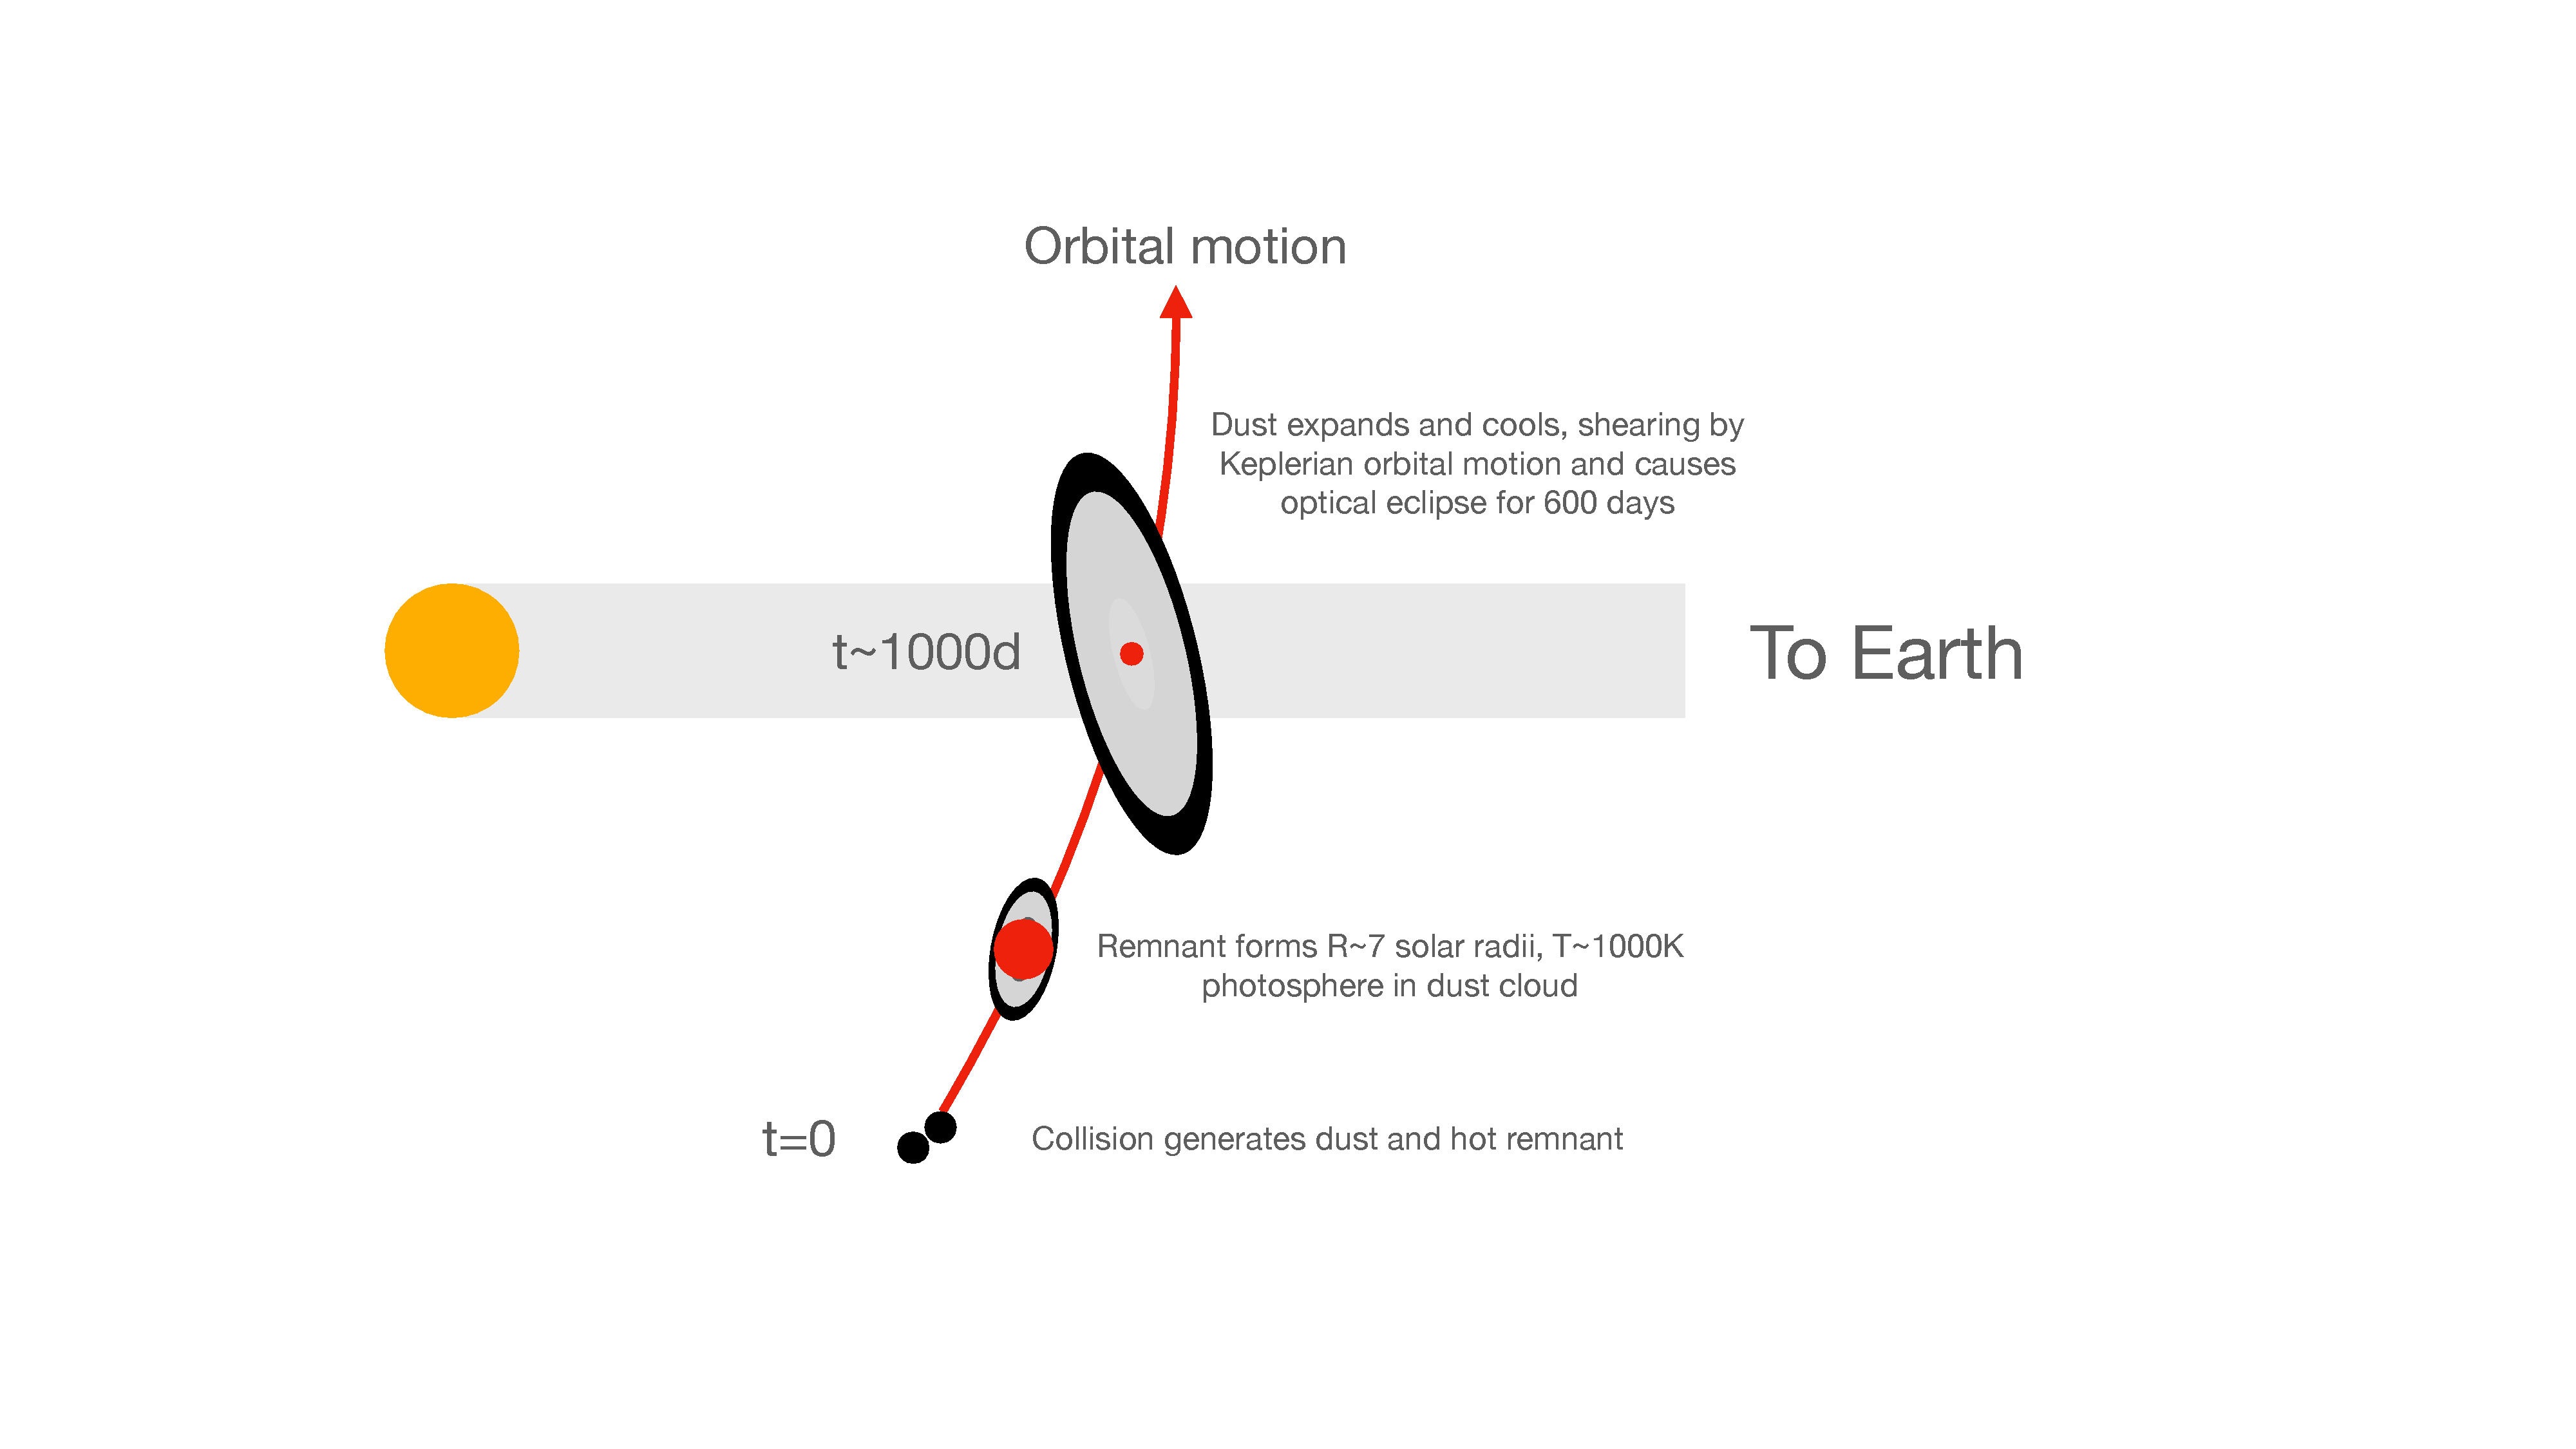
\includegraphics[width=1\textwidth]{asassn-21qj-cartoon.pdf}
    \caption{Sketch of the hypothesis for the observations seen towards ASASSN-21qj.
    %
    At $t=0$, the collision occurs, producing a cloud of debris that expands and cools.
    %
    Material close to the remnant is heated by its luminosity, generating the 1000\,K infrared emission.
    %
    Around 1000 days later the expanding cloud crosses the line of sight between the star and the Earth, generating the optical light curve.}
    \label{fig:hypothesis}
    %\script{blueing.py}
\end{figure}


First, the IR flux increase and the optical dimming might be unrelated, coincidental phenomena. 
%
For example, one debris disk at 0.1~au passively heated to 1000\,K producing the IR emission and another disk further from the star that transited \asas.
%
This explanation is unsatisfactory because both IR flux increases and dimming events are rare.
%
Mid-IR excesses are exceptionally rare among main-sequence stars \cite[1:10,000,][]{2013MNRAS.433.2334K}, and still uncommon for young stars \cite[1:100,][]{2013MNRAS.433.2334K}, and no star has previously shown a sizeable increase starting from no excess. A single case of a disappearing mid-IR excess has been seen, which remains largely unexplained \cite{2012Natur.487...74M}.
%
Similarly, optical dimming events are rare for main-sequence stars, for example only one was seen to undergo dust-related optical dimming with Kepler main mission, which observed 150,000 stars for four years \cite{2016MNRAS.457.3988B}.
%
Both optical and IR variability are independently less than 1\% probabilities for a given star, so for \asas~to show both by chance is at best a 0.01\% probability, and probably much lower.

Another possibility is that both the IR and optical features are produced by a single debris disk at about 0.1\,au from the star.
%
At such a close distance, any dust clumps would initially produce periodic eclipses on the timescale of days \citep{2019MNRAS.488.4465G} before being sheared into an azimuthally symmetric structure in months, so the occultation of the star would need to be be related to changes in the vertical structure of a near edge-on post-collision disk, for example by dynamical ``stirring'' of debris by impact remnants \cite{1992Icar...96..107I}.
%
The optical depth of the disk must then decrease due to ongoing collisional depletion to explain the slow return to pre-transit levels of optical flux and gradual decrease in IR flux.
%
Three issues with this model are that 1) the disk must have precisely the right geometry to slowly occult the star as the scale height increased, and must coincidentally become optically thin, 2) there is no apparent change in dust temperature, which would be expected as the optical depth decreases and the warmer inner disk becomes visible, and 3) significant optical variation is seen three years after the putative collision, so any initially created clumps would already have sheared out.
%
Newer clumps must contribute of order 50\% of the dust area to explain the large variations around 59500\,MJD, but the IR flux shows a gradual decline rather than any strong variation that would be associated with clump creation.
%
A fourth, but less critical issue, is that the inferred clump velocities are not as high as they could be for transiting structures at 0.1\,au, which should result in transverse velocities of up to 100\,km\,s$^{-1}$.

\subsection*{SPH collision simulations}

To provide some more insight into the collision scenario, we performed impact simulations using the SWIFT smoothed particle hydrodynamics (SPH) code \cite{Schaller2016,Schaller2018,Kegerreis2019}.
%
Extended Data Figure \ref{fig:SPH} shows a collision between two 25~$M_{\rm Earth}$ (Earth-mass) planets at 45.77~km~s$^{-1}$ (1.4~$v_{\rm esc}$, escape velocity neglecting the atmosphere) at an impact parameter of 0.4 (an impact angle of 23.6$^\circ$).
%
The colliding bodies were 22.5\% rock \cite[forsterite,][]{Stewart2019forsteriteEOS,Stewart2020_key_req_EOS}, 67.5\% water \cite{Senft2008}, and 10\% H/He \cite{Hubbard1980} by mass.
%
2.1$\times10^6$ particles were used in the simulation.
%
To make simulations with high resolution numerically tractable, SWIFT imposes a maximum smoothing length that, in effect, imposes a minimum density for particles in the simulation ($\sim30$~kg~m$^{-3}$ for the simulation shown here). 
%
The bound post-impact material is spread over hundreds of Earth radii following the collision, illustrating that giant impacts can produce very large post-impact objects. 

However, for the massive and highly extended bodies produced by collisions between super-Earths and mini-Neptunes, a large fraction of the post-impact body is at the minimum density (green particles in lower right panel in Figure~\ref{fig:SPH}).
%
SPH simulations therefore likely underestimate the extent of such post-impact bodies, and further work is needed to fully quantify the size of post-impact bodies produced in different impacts.

\begin{figure}
    \centering
    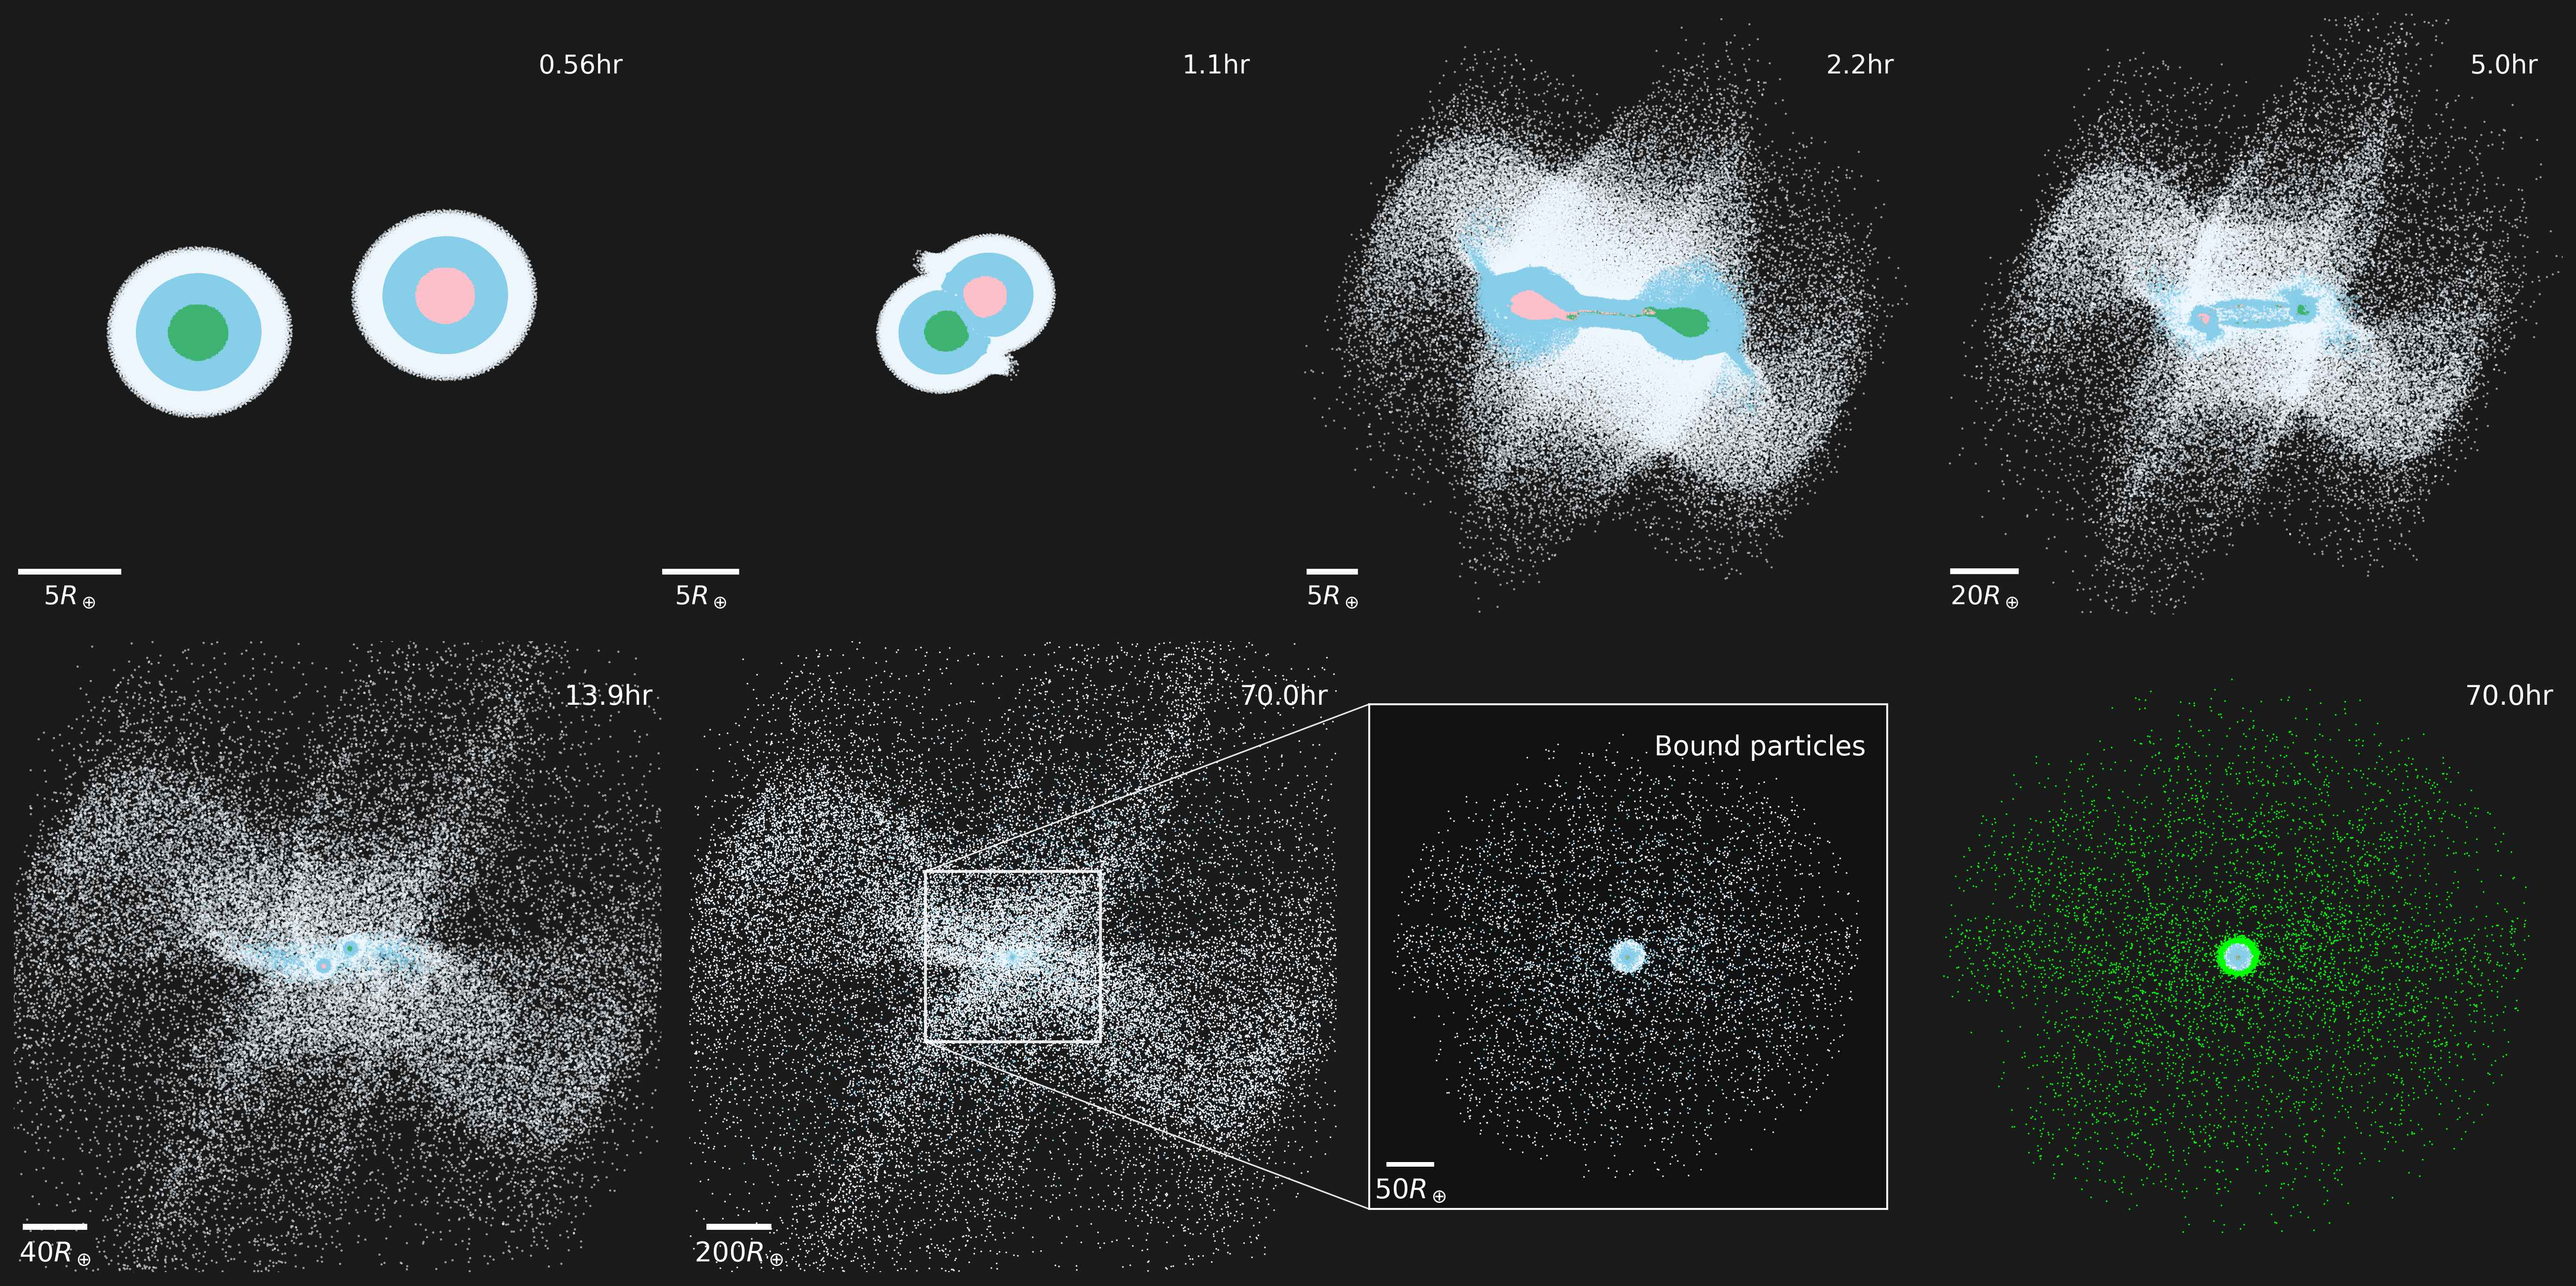
\includegraphics[width=1.0\textwidth]{final_v2_less0d029.png}
    \caption{Simulations of the formation of a post-impact body.
    %
    Giant impacts between super-Earths and mini-Neptunes can produce post-impact bodies hundreds of Earth-radii across, comparable to that required to produce the observed infrared flux. With the exception of the lower right panel, particles are colored by their material (forsterite, water, or a H$_2$-He mixture moving outwards in the initial bodies) and whether they came from the impactor or target (see top left panel). The final two panels show just the mass bound to the primary remnant which has a mass of 48.4~$M_{\rm Earth}$. In the final panel, particles that are at the minimum density imposed by the code are colored in green.}
    \label{fig:SPH}
 %   \script{fvsr.py}
\end{figure}


\subsection*{Post-impact body cooling calculations}

How the emission from a post-impact body would evolve with time is highly dependent on the initial mass distribution and thermal state of the body, and the balance between radiative cooling, viscous spreading, and mass and angular momentum transport by condensates \cite{Lock2017,Lock2018moon,Lock2020}. 
%
Given the limitations of SPH simulations (see above) it is not possible to accurately determine the initial structure of post-impact bodies in the relevant regime.
%
To explore a range of possible evolution pathways, we have calculated the evolution of post-impact bodies with different power-law surface density profiles, $\Sigma$, profiles, under the limiting case that radiative cooling and condensation of the vapor is the single driver for evolution of the structure. 
%
We chose a power-law surface density profile as it can straightforwardly cover the wide range of surface density profiles expected after super-Earth/mini-Neptune collisions, based on that found in impact simulations between lower-mass, terrestrial bodies \cite{Lock2017,Canup2001,Canup2012,Cuk2012,Rufu2017,Reufer2012}. 
%
The surface density profile is given by:
%
\begin{equation}
\Sigma=\begin{cases}
\Sigma_0, & \text{if } r_{xy}\leq R_{\rm c}\\
\alpha r_{xy}^{\beta}, & \text{if } R_{\rm c} > r_{xy}\leq R_{\rm emit}\\
0, & \text{if } r_{xy}> R_{\rm emit}
\end{cases}   
\label{eqn:sigma}
\end{equation}
%
where: $r_{xy}$ is the distance from the rotation axis; $R_{\rm c}$ is the outer radius of a constant surface density central region, roughly analogous to the corotating regions seen in Earth-mass synestias \cite{Lock2017,Lock2018moon}; $\Sigma_0$ is the surface density of the central region; $\beta$ is the power law exponent; and $R_{\rm emit}$ is the initial emitting radius. Imposing surface density continuity gives
%
\begin{equation}
    \alpha=\Sigma_0 R_{\rm c}^{-\beta} \; .
\end{equation}
%
We can determine $\Sigma_0$ by fixing the mass of the body, 
%
\begin{equation}
    M_{\rm p} = \int_0^{R_{\rm c}}{2 \pi r'_{xy} \Sigma_0 dr'_{xy}} + \int_{R_{\rm c}}^{R_{\rm emit}}{2 \pi r'_{xy} \Sigma(r'_{xy}) dr'_{xy}} \; ,
\end{equation}
%
which can be solved to give:
%
\begin{equation}
\Sigma_0=\begin{cases}
\frac{M_{\rm p}}{\pi \left [R_{\rm c}^2 + 2 R_{\rm c}^{-\beta} \left ( \ln{R_{\rm emit}}-\ln{R_{\rm c}}\right ) \right ]}, & \text{if } \beta=-2,\\
\frac{M_{\rm p}}{\pi \left [R_{\rm c}^2 + \frac{2 R_{\rm c}^{-\beta}}{\beta+2} \left ( R_{\rm emit}^{\beta+2}-R_{\rm c}^{\beta+2}\right ) \right ]}, & \text{otherwise.} 
\end{cases}
\end{equation}
%
The time taken for a given region of the structure to cool to the point that a sufficient fraction of material is condensed for the temperature to drop below the condensation-buffer (see above) and so the emitted flux to drop is given by
%
\begin{equation}
    t_{\rm cool} (r_{xy})=\frac{l f(r_{xy}) \Sigma(r_{xy})}{\sigma T^4_{\rm emit}}
\end{equation}
%
where $f$ is the initial vapor fraction at that radius, $l$ is the latent heat of vaporization of the material (here we have taken the limiting case of pure water $l=2.256\times 10^6$ \cite{Chase1998}, but the addition of silicates could make the latent heat much larger), $\sigma$ is the Stefan–Boltzmann constant, and $T_{\rm emit}$ is the emission temperature. Figure~\ref{fig:Hill_Bondi_R} shows example evolutions of the emission from a post-impact body using this model for different parameters (solid lines). Results of a modified model where the initial surface density (by the addition of a constant parameter to Equation~\ref{eqn:sigma}) is forced to be zero at $R_{\rm emit}$ are shown as dashed lines.

% The colour-dependent dimming yields an indication of dust grain size; Figure \ref{fig:blueing} shows that the relative extinction is $A_B/A_V \approx 1.3$ and $A_i/A_V \approx 0.6$. These ratios are consistent with those seen for interstellar dust, indicating that i) the occulting dust is probably not significantly optically thick, and ii) that the typical grain sizes are sub-micron in size \citep[e.g. the dominant ISM grain sizes assumed by][are 1100 to 1430 $\AA$]{1977ApJ...217..425M}. While conversion from occulted surface area to mass has many uncertainties, not least that not all of the dust may not have passed in front of the star, nor is the transverse velocity of the material known, we may still make a ball-park estimate. From the optical light curve we assume that the star was uniformly dimmed by 1\,mag for 300\,d. Assuming that the transverse velocity of the dust is $v$\,km\,s$^{-1}$, the length of the cloud is $0.17 v$\,au, so for a circular orbit at 10\,au the length would be 1.7\,au. Now assuming that the star has the same radius as the Sun, that the dust covers the star entirely and extends no `higher' than the star (i.e. all dust is accounted for), the dust surface area is 0.008\,au$^2$. The conversion from surface area to mass for a single grain size requires multiplying by a factor $4r \rho$ (where $\rho$ is  density), so assuming 0.1\,$\mu$m particles  with density $\rho=5$\,g\,cm$^3$ yields a mass of $4 \times 10^{17}$\,kg. This mass is 3 orders of magnitude greater than Halley's comet, and 3 orders of magnitude smaller than Ceres. Given that an event that generates such levels of dust will not create particles of only very small sizes, the implication is that the true mass is significantly greater, probably by several orders of magnitude. The mass is however significantly smaller than the estimated impactor masses.

% We can also estimate the dust surface area and mass from the infrared excess, which requires far fewer assumptions, as the surface area is simply $4 \pi r^2 L_{\rm disk}/L_\star$. If we assume the dust is close to the star, e.g. 0.1\,au, the area is then 0.004\,au$^2$, similar to the above estimate. If the dust is at 10\,au, the area is 40\,au$^2$. The large difference between the area estimates suggests either that most of the material did not transit the star, or that the implicit assumption here that the dust is heated by the star is false.

%\subsection*{Transverse velocity of the dust cloud}



% \subsection*{Frequency analysis of the light curve}

% %To search for signs of periodicity within the light curve before and during the eclipse, we perform a Lomb-Scargle analysis over two epochs indicated with the blue and orange regions in the upper panel of Figure\~\ref{fig:starlombscargle}.
% %
% %The resultant periodograms are shown in the lower two panels of Figure\~\ref{fig:starlombscargle}, with the lower panel showing a zoom in from 0 to 50 days and the middle panel showing periodicities from 0 to 150 days.
% %
% We look for any periodicities that could be associated with orbital motion around the star, so we look at the periodogram for signals of 1 to 150 days period during the eclipse.
% %
% As a comparison, we overplot the periodogram for the pre-eclipse light curve as the blue curve in the middle panel. 
% %
% There is some power seen at 40 days which is present in the pre-eclipse light curve, with some (non-significant) periodicities at longer periods.

% Looking for periodic stellar activity, the periodogram for the pre-eclipse light curve is shown from 0 to 50 days in the lower panel.
% %
% Here we see significant periods at around 6.5 and 11 days, which we attribute to light curve modulation caused by starspots rotating in and out of view. 


% \begin{figure*}
%   \begin{centering}
%   \includegraphics[width=\textwidth]{scale_combined_photometry.pdf}
 %     \caption{Photometry from the optical bands of the eclipse scaled arbitrarily so as to combine the light curves into a ``gray'' light curve.
      %
%      The axis is inverted to show Absorption.
%              }
%              \label{fig:allphot}
              %\script{plot_scale_combined_photometry.py}
              %\end{centering}
       %\end{figure*}

% \section{Discussion}\label{sec:discussion}

% We have two separate observed phenomena that occur within 1000 days of each other.
% %
% Firstly, NEOWISE W1 and W2 photometry shows an approximate doubling of flux in both wavebands, with the longer wavelength showing a greater increase.
% %
% The pre-brightening colour is consistent with the colour expected for a star of this spectral type.
% %
% Observations from the optical bands between the two epochs where the NEOWISE increase occurred have a much higher temporal cadence, but they do not show any corresponding increase in flux.
% %
% This infrared only increase is consistent with a dust generating event, such as the collision of a planetoid with another planetoid or a terrestrial planet.
% %
% This interpretation is also supported by the reddening of the star during the optical dimming, if we assume that both the optical and IR flux variations are caused by the same dust cloud, then we  (discussed further below).
% %
% The resultant dust cloud has a considerably larger surface area than the progenitors (which were not visible before the IR flux increase), and this dust cloud is then heated by some luminosity source.
% %
% Typically the host star heats circumstellar dust, but we consider alternative possibilities below.
% %
% The temperature of the dust cloud can be estimated from spectral energy distribution (SED) measured towards the stellar system. A post-increase SED is shown in Figure \ref{fig:sed-after}, using WISE data from the first five post-increase epochs, for which the best-fit dust temperature is $910 \pm 50$\,K. This temperature is consistent with those derived from the time series, though more precise because the data have been averaged.

% \begin{figure}
%     \centering
%     \includegraphics[width=1\textwidth]{asassn-21qj-after.pdf}
%     \caption{SED of \asas~after the IR flux increase. The blue line shows the stellar photosphere model, the red line the dust model (a blackbody), and the orange the total.}
%     \label{fig:sed-after}
% \end{figure}



% \begin{figure}
%     \centering
%     \includegraphics[width=0.8\textwidth]{fvsr.pdf}
%     \caption{Model-independent constraints in terms of dust fractional luminosity ($L_{\rm dust}/L_\star$) and stellocentric radius or temperature.
%     %
%     The dot shows the location of the dust from an SED fit to both NEOWISE bands, and the curved line shows cooler dust that is consistent with a constraint of a single temperature blackbody fit to the WISE W2 flux.
%     %
%     The diagonal line shows the upper limit from the ALMA non-detection.
%     %
%     The vertical dotted line shows an approximate lower radial limit on the dust location based on the transit duration.
%     %
%     The dashed line a lower radial limit based on the delay between the IR flux increase and optical transit.
%     %
%     The vertical solid line shows an upper radial limit based on the optical light curve gradients.}
%     \label{fig:constr}
%  %   \script{fvsr.py}
% \end{figure}

% This increase occurred between MJD \variable{output/t_before.txt} and MJD \variable{output/t_after.txt} dates, a period of approximately \variable{output/t_duration.txt} days.
%
% Subsequent NEOWISE measurements show an approximately constant excess flux for XXXX days, followed by a decrease from XXXX to XXX.

% We fit a blackbody SED to the excess flux in the two NEOWISE bands for each of the epochs.
%
% Assuming grey emission (where $\upsilon(\lambda)\approx \upsilon$) we obtain an effective temperature of $_{IR} = 1000\pm XXX$K, and $F_{IR}/F_{star}=0.03$.
%
% Given the near-Solar luminosity of the star, this temperature implies a distance of approximately 0.1\,au if the material absorbs and emits as a blackbody, and of order a few times more distant if it is micron-sized dust (e.g. Pawellek). 
%
% The sudden onset of the IR flux within 155.21 days followed by a constant level of flux implies that the dust cloud reaches a (quasi) steady state within 6 months, though could be optically thick or thin.
%
% Regardless, the dust distribution has had to expand such that 0.03 of the solid angle around the star was subtended by dust and re-radiated in the IR.
%
% An estimate for the surface area $A_{IR}$ of the dust can be estimated from $A_{IR}/(4\pi r_{IR}^2) = 0.03$ which leads to:

% $$A_{IR}=0.38 r_{IR}^2$$ 

% where $r_{IR}$ is the distance of the dust from the star.

%%Hansen collision of terrestrial planet with scattered moon \cite{2022MNRAS.tmp.2636H}

%\subsection*{Hypothesis 1: Two unrelated phenomena} 
% \subsection*{Notes on collision aftermath} 


% \begin{figure*}
% \begin{centering}
% \includegraphics[width=\textwidth]{asassn-21qj-hypotheses.pdf}
% \caption{Cartoon of the three hypotheses under consideration. At $t=0$ two or more rocky bodies collide to produce an expanding cloud of dust.
% %
% At approximately $t=900$\,d the optical transit begins.
% %
% The system is seen from the vantage point of above and looking down onto the components.
% %
% The observing line to the Earth is straight downwards off the page.
% }
% \label{fig:hypo}
% \end{centering}
% \end{figure*}

%\subsection*{Hypothesis 3: Aftermath of a collision between two planets} 

% Collisions between planet-sized bodies, known as giant impacts, are a common occurrence in planet formation \cite{Raymond2013,Izidoro2015,Schlichting2018a,DAngelo2018} and can also occur as a result of dynamical instabilities in older systems \cite{Kaib2016,Izidoro2017}.
% %
% In our own solar system, giant impacts are thought to explain, among other things, the large iron core of Mercury \cite{Benz1988}, the formation of Earth's Moon \cite{Cameron1976,Hartmann1975}, and the axial tilt and heat flow of Uranus \cite{Kegerreis2018,Slattery1992}.
% %
% Giant impacts have a variety of outcomes but typically result in one or more massive bodies (known as remnants or post-impact bodies) and debris of a range of sizes that is unbound to any one of the remnants.
% %
% A possible explanation of our observations is that we are seeing thermal emission from a substantially heated post-impact planetary body and the subsequent transit of the cooled impact ejecta. 
% %
% Such a scenario would allow for production of the observational signatures with a single event that would be a relatively common occurence in such a young system as \asas{}.
%
%We will now consider each component of the observed signal in turn.


% \subsubsection*{The post-impact body as a source of the initial observed brightening}

% Giant impacts are one the most energetic events planets experience.
% %
% For example, the kinetic energy of a giant impact that formed a Neptune-mass body is on the order of $10^{33}$-$10^{34}$~J, enough to vaporize the colliding bodies several times over.
% %
% A significant fraction of this kinetic energy gets dissipated as heat in the post-impact body \cite{Carter2020,Lock2020} and giant impacts typically leave the post-impact body substantially melted and vaporized \cite{Nakajima2015,Lock2017,Carter2020}.
% %
% The large torques exerted in the impact also generally produce rapidly rotating post-impact bodies \cite{Lock2017,Rufu2017}.
% %
% Due to their low density and rotational flattening, post-impact bodies can be hundreds of times larger than the bodies that collided to produce them \cite{Lock2017}. Such a body may be large enough and hot enough to explain the increased luminosity of \asas{} at $\sim$1000~K.

% The signatures of post-impact bodies in astronomical observations has not been explored in any depth.
% %
% Particularly for more massive bodies, resolution and computational efficiency limitations of giant-impact simulations makes resolving the low-density regions of post-impact bodies, at which the body would become optically thin, extremely challenging
% %
% Preliminary simulations of high-energy impacts between super-Earth and mini-Neptune -like  bodies using the SWIFT hydrodynamics code \cite{Schaller2016,Schaller2018,Kegerreis2019} with a density floor of $\sim$10$^{-2}$~kg~m$^{-3}$ showed that the post-impact bodies could be hundreds of Earth radii ($R_{\rm Earth}$) in radius.
% %
% Such an object radiating at $\sim$1000~K would produce a flux comparable to the 0.034~$L_*$ inferred from our observations. 

% Independent of a particular impact or simulation, fundamental limits can be placed on the possible size of post-impact body by considering the Hill and Bondi radii.
% %
% The Hill radius is the distance from an object in which the gravity of that object dominates over that of the star and can be approximated by
% %
% \begin{equation}
%     R_{\rm H}=a \left ( \frac{M}{3M_*}\right )^{\frac{1}{3}} \; ,
% \end{equation}
% %
% where $a$ is the semi-major axis of the object from the star, $M$ is the mass of the object, and $M_*$ is the mass of the star.
% %
% Any post-impact structure must be smaller than the Hill sphere of the body.
% %
% Furthermore, for vapor to be bound to a body it must be within the Bondi radius of the body for the temperature of the gas.
% %
% The Bondi radius is given by
% %
% \begin{equation}
%     R_{\rm B}=\frac{2 G M}{c_s^2} \; ,
% \end{equation}
% %
% where $G$ is the gravitational constant, and $c_s$ is the isentropic sound speed which, for an ideal gas, is 
% %
% \begin{equation}
% c_s = \sqrt{\frac{\gamma k_{\rm B} T}{m_a}} \; ,
% \end{equation}
% %
% where $\gamma$ is the ratio of specific heat capacities for the gas, $k_{\rm B}$ is Boltzmann's constant, $T$ is temperature, and $m_a$ is the molar mass of the gas.
% %
% Any vapor in the structure can only remain bound if it is within the Bondi radius.
% %
% If the structure is a mixture of vapor and condensates (i.e., liquid droplets or solid dust) then the vapor fraction outside the Bondi radius would be lost, acting as an open-system. 

% Figure~\ref{fig:Hill_Bondi_R} shows the Hill radii for different mass bodies at different distances from ASASSN-21qj (solid lines) and the Bondi radius for H$_2$, H$_2$O, SiO, and SiO$_2$ (dotted lines).
% %
% The black dashed line also shows the radius of the body required to explain the observed flux at 1000~K ($\sim0.7R_*$, Section~\ref{sec:obs}).
% %
% The Hill radius of bodies more than approximately an Earth-mass are large enough to accommodate a post-impact body large enough to produce the observed thermal emission, although this rises to tens of Earth masses at 1~au.
% %
% For heavier gases (e.g., H$_2$O, SiO, and SiO$_2$), vapor would be bound from the emitting body if it was more than a few Earth masses, although a body of more than $\sim35M_{\rm Earth}$ would be required to hold hydrogen vapor.
% %
% Therefore, theoretically, a post-impact body of a few Earth-masses at a few au from the star could be large enough to explain the observed thermal emission from a surface that was dust or a mixture of dust and vapor.
% %
% However, further work is required to probe what impacts could produce such a large structure.



% Creation of a post-impact body large enough to explain the observed data would most likely require a high-energy impact with a total colliding mass of several to tens of Earth-masses.
% %
% Such a high energy impact, given sufficient angular momentum, could result in the formation of a synestia - a hypothesised class of structures thought to be a common outcome of giant impacts \cite{Lock17}.
% %
% If confirmed, detection of a synestia would transfer synestias from a theoretical prediction into a newly-accessible class of planetary object.

% One key line of evidence that suggests we have observed a post-impact structure is the relatively constant emission temperature.
% %
% At high pressures in the interior, post-impact bodies generated by high-energy impacts are typically mostly liquid.
% %
% The structure then transitions with decreasing pressure, and increasing distance from the center, to supercritical fluid, then vapor, and then a mixture of vapor and condensates \cite{Lock2017,Lock18,Caracas2023}.
% %
% At low enough pressure the structure becomes optically thin and the temperature at this point would set the temperature of thermal emission and energy loss from the post-impact body.
% %
% \cite{Lock18} suggested that the emission temperature of a post-impact body is set by the thermodynamic properties of the material that make up its outer regions, and so remains constant for many years as it cools.
% %
% They suggested that the emission from a post-impact body was primarily from a cloud layer, above which the opacity and density of the gas/condensate mixture is not large enough to make the structure optically thick.
% %
% For the rocky post-impact bodies that \cite{Lock18} studied, the dew point (the onset of significant condensation approaching the boundary from high temperatures) and bubble point (the onset of significant vaporization approaching the boundary from low temperatures) are close \cite[within $\sim 100$~K,][]{Lock18,Fegley2023_BSE_cond} at the low pressures of the outer potions of a post-impact body at $\sim2300$~K.
% %
% Such a high temperature is inconsistent with our observations, but the mechanisms by which the radiative temperature is set by the thermodynamics of a material would likely also apply in post-impact bodies with different compositions, resulting in different radiative temperatures. 

% It is thought that water and other ices/gases could be key components of many planets [CITE?].
% %
% Due to their relatively low densities, these components would be concentrated at lower pressures in planetary bodies, and therefore susceptible to heating by giant impacts.
% %
% Water has a vaporization temperature that is on the order of a few 100~K, depending on pressure, much lower than silicates \cite[e.g.,][]{Wagner2002}.
% %
% At the low pressures near the photosphere of a post-impact body, the condensation temperature of pure water would in fact be too low, $\sim250$~K, to explain the observed $\sim$1000~K emission we observe.
% %
% However, a multi-component mixture of water and rock (and other constituents) would have bubble and dew points intermediate between that of water and silicates.
% %
% For example, the addition of small amounts (on the order of 10$^{-3}$ mole fraction) of water may reduce the bubble and dew points for rocky post-impact bodies by order 100~K \cite[][c.f., \cite{Fegley2023_BSE_cond}]{Lock18}.
% %
% For a certain chemical mixture of vaporized rock and ices in the outer regions of a post-impact body, the bubble and dew points would be $\sim$1000~K and, following the same logic as \cite{Lock18}, the emission temperature would also be set at $\sim$1000~K by the condensation of clouds.
% %
% Note that, in this scenario, a post-impact body with an emission temperature of $\sim$1000~K is not a general outcome of giant impacts, but rather a function of the specific composition of the outer regions of the post-impact body.
% %
% Physical chemical studies of the vaporization of ice-rock mixtures is required to further understand the relation between composition and emission temperature.
% %
% Therefore, a collision between bodies that were combinations of rock, ice, and iron, could produce a post-impact body with a radiative temperature of $\sim$1000~K that would remain consistent for many years as dictated by the thermodynamics of the hot water-rock mixture.  

% The temporal variation of the flux from a post-impact body depends on how the size of the body changes with time.
% %
% The evolution of the structure of post-impact bodies is governed by a number of competing factors \cite{Lock18,Lock2019pressure,Lock2020}.
% %
% Cooling of the outer region by radiation leads to condensation of the vapor and reduction in the pressure support of the structure, promoting contraction.
% %
% Conversely, viscous spreading of the structure and dragging of the gas by in-falling condensates would both act to transport angular momentum and mass outwards in the post-impact body leading to expansion.
% %
% Due to the high radiative temperature of silicate-dominated post-impact bodies, \cite{Lock18} found that for Moon-forming impacts cooling dominated over viscous spreading and the post-impact body contracted rapidly, on a timescale of years.
% %
% As the radiative surface area was greatest earlier in evolution, the rate of contraction decreased with time.
% %
% This is not we observe in the case of \asas{}, where the flux stays relatively constant for hundreds of days and then slowly decreases.
% %
% The post-impact body we observe is radiating at a much lower temperature than those considered by \cite{Lock18}, and the balance of different processes will be different.
% %
% It would take tens to hundreds of years to radiate away the impact energy from an impact that formed a tens of Earth-mass body, even at the maximum flux observed, and it is therefore very feasible that a post-impact body could remain close to its maximal extent for a long period, with radiative cooling balanced by viscous spreading.
% %
% Eventually, however, radiative cooling would likely `win', leading to a decrease in the size and hence luminosity of the body, as we observe.
% %
% Further work is required to understand how post-impact bodies of different compositions and lower radiative temperatures would evolve in order to test whether our observations are consistent with a post-impact body.

% It is important to consider that we may not have directly observed the vapor pressure-supported post-impact structure, but rather a population of dust injected into orbit around the body.
% %
% This dust would be heated by radiation from the post-impact body, potentially at higher temperatures higher than the observed 1000~K.
% %
% The emission temperature of the dust could be limited by heating to the bubble point of the material, as substantially more energy is required to heat the dust to higher temperatures \cite[see discussion of the silicate vaporization buffer in ][]{Lock18}.
% %
% Over time, this dust would be swept out of the bodies gravity well by radiation pressure, an effect which could potentially not affect the outermost, emitting volume of dust for some time after the impact.
% %
% Dust that was swept away from the post-impact body would cool quickly as the radiative flux from the post-impact body reduced.
% %
% The dispersal of the dust would lead to the decrease in the extent and luminosity of the body, as observed.
% %
% As above, further work is required to investigate this possibility.


% Observation of a post-impact body would be the first detection of its kind and would offer a fascinating insight and constraint on the mechanisms of planet formation.
%
% It is therefore necessary to obtain rigorous confirmation of any such interpretation of observations.
%
% Long wavelength spectroscopy could reveal emission or absorption features of silicates or ices from the post-impact body, confirming the existence of a water/rock post-impact body in the system.
%
% Furthermore, tracking of the evolution of the thermal emission over time by more sensitive instruments, such as JWST, could be used to test future models of the evolution of post-impact bodies to test the feasibility of our proposed interpretation. 



%\subsubsection*{Theoretical limits on the size of a post-impact body}

% The possible size of a post-impact body is limited by the Hill and Bondi radii for a body of a given mass. 
% %
% The Hill radius of a body is given by
% %
% \begin{equation}
%     R_{\rm H}=a \left ( \frac{M}{3M_*}\right )^{\frac{1}{3}} \; ,
% \end{equation}
% %
% where $a$ is the semi-major axis of the object from the star, $M$ is the mass of the object, and $M_*$ is the mass of the star.
% %
% Any post-impact structure must be smaller than the Hill sphere of the body.
% %
% Furthermore, for vapor to be bound to a body it must be within the Bondi radius of the body for the temperature of the gas.
% %
% The Bondi radius is given by
% %
% \begin{equation}
%     R_{\rm B}=\frac{2 G M}{c_s^2} \; ,
% \end{equation}
% %
% where $G$ is the gravitational constant, and $c_s$ is the isentropic sound speed which, for an ideal gas, is 
% %
% \begin{equation}
% c_s = \sqrt{\frac{\gamma k_{\rm B} T}{m_a}} \; ,
% \end{equation}
% %
% where $\gamma$ is the ratio of specific heat capacities for the gas, $k_{\rm B}$ is Boltzmann's constant, $T$ is temperature, and $m_a$ is the molar mass of the gas.
% %
% Any vapor in the structure can only remain bound if it is within the Bondi radius.
% %
% Figure~\ref{fig:Hill_Bondi_R} shows the Hill and Bondi radii for different bodies and gases, the implications of which are discussed in the main text.



%\subsubsection*{Impact ejecta as the source of the transiting material}

% Giant impacts can produce significant amounts of debris that is ejected from the gravitational well of the colliding bodies onto orbits that are largely different than, but cross, that of the remnants.
%
% For example, proposed single Moon-forming impacts produce one to several percent of the colliding mass as debris \cite{Canup2001,Canup2012,Cuk2012,Reufer2012,Lock18}.
%
% The transit of the star we observe, delayed from the onset of the increase in thermal emission, could be caused by the transit of this impact debris. 

% % Material ejected from impacts can have a wide range of sizes, from sub-micron dust to planetesimals of many tens to hundreds of kilometers \cite{Benz2008_Mercury_book,Leinhardt2012,Leinhardt2015,Carter2020a}, and often contains the most highly heated material in the impact.
%
% For sufficiently high impact velocities ($>1$~km~s$^{-1}$ for water ice, and $>8$~km~s$^{-1}$ for forsterite) a substantial fraction of this material is vaporised \cite{Stewart2008,Davies2017,Davies2020,Carter2020a}.
%
% Shearing of droplets by the vapor, and rapid cooling and condensation of the vaporised material would rapidly produce a population of small dust grains and solid spherules.
%
% The size distribution of this fraction of the impact debris is uncertain, due to difficulties in modelling nucleation and droplet breakup in shearing flows, but previous work suggests that such debris could range from 10$^{-8}$-10$^{-1}$~m \cite{Benz2008_Mercury_book,Johnson2015,Asphaug2011} in radius.
%
% Our observations suggest that the transiting dust cloud we observe is made optically thick by micron grains, which is firmly consistent with these previous estimates for the sizes expected for impact debris.

%Debris ejected from an impact would be injected into a range of orbits and would then be further spread out by Keplerian shear..... 

% \begin{figure*}
% \begin{centering}
% \includegraphics[width=\textwidth]{expansion_rate.pdf}
% \caption{The instantaneous velocity of the cloud crossing the line of sight to the star, and in the lower panel, the evolution of the cloud's expansion with time.
% %
% %The time since the collision is along the x-axis, and the distance along the orbit of the cloud is on the y-axis.
% %
% The collision occurs at $t=0$ and the outermost bound of the cloud expands from the centre of the collision point with a velocity $v_{e}$.
% %
% The leading edge of the cloud crosses the line of sight between the Earth and the star at $t_{s}$ with the cloud continuously expanding along its orbital motion during the eclipse, with the trailing edge leaving the line of sight at $t_{e}$.
% %
% The distance from the collision point to the centre of the cloud transiting the star is $d_{cs}$.
% }
% \label{fig:collisionpoint}
% \end{centering}
% \end{figure*}

% We can estimate some properties of the observed debris by using a simple model.
% %
% The geometry of an expanding cloud of debris is shown in Figure \ref{fig:collisionpoint}.
% %
% We define the time of the collision at $t=0$ and the resultant debris cloud expands with a expansion velocity of $v_{e}$ for the fastest debris whilst moving along its orbit with velocity $v$.
% %
% The leading edge of the cloud begins to cross the line of sight to the star at $t_s$, expanding as it transits the star, then the trailing edge leaves the disk of the star at $t_e$.
% %
% As the cloud expands during the transit, the instantaneous velocity crossing the stellar line of sight changes linearly from $v+v_e$ to $v-v_e$.
% %
% The distance from the collision point to the stellar line of sight is $d_{cs}$ and the time at which the midpoint of the disk crosses the stellar line of sight is $t_{cs}$, typically before the mid-point of the eclipse $(t_{e}-t_{s})/2$.
% %
% The diameter of the cloud at time $t$ is then simply $2vt_{cs}$.

% Writing equations for the time and velocity at the trailing and leading edges of the cloud and eliminating $d_{cs}$ from these two equations leads to the ratio of the expansion velocity to the orbital velocity: 

% $$\frac{v_e}{v}=\frac{t_e-t_s}{t_e+t_s}$$
% t=58150.
% ts=59200-t
% te=59800-t
% (te-ts)/(te+ts)
% 0.22
% ts,te
% Out[7]: (1050.0, 1650.0)
% %

% Taking approximate times for the two times $t_s=1050$ d and $t_e=1650$ d leads to $v_e/v=0.22$.


%If we assume that the dust cloud expanded from a point source out into a star-facing circular optically thin disk with area $A_{IR}$ and radius $r_{IR}$ in a time $t_{IR}$ (where this time has an upper limit of 6 months corresponding to the duration between the NEOWISE epochs), then we can estimate a linear velocity $v_{IR} t_{IR} = r_{IR}$ for the expansion of the cloud of:

%$$v_{IR} = \frac{r_{IR}}{t_{IR}} = \frac{0.35 r_{IR}}{t_{IR}} = $$
%# A_{IR} / 4 pi (a_{IR})2 =  pi r_{IR}^2 / 4 pi a2 = 0.03
% r2 / (4a2) = 0.03
% $r_{IR} = 2a_{IR} sqrt(0.03)$

%A figure showing the temperature dependency is is Figure~\ref{fig:veloc_cons}.

%\begin{figure}
%%    \begin{centering}
 %   \includegraphics[width=0.5\textwidth]{velocity_constraints.pdf}
 %   \caption{Circular velocity as a function of semimajor axis, and the effective temperature of dust as a function of semi-major axis.
%              }
%    \label{fig:veloc_cons}
%    \script{calc_velocity_bounds_plots.py}
%    \end{centering}
%\end{figure}

%Irregular collisions \cite{Genda15}.

% One advantage of this hypothesis is that we are no longer tied to surface area/distance from star dichotomy, and that the derived circular velocities from the light curve gradients can be made consistent with an orbit out at Jupiter/Saturn distances.
% %
% We therefore require a new energy source to heat the dust - we note that the gravitational binding energy of two large terrestrial planets colliding can produce enough energy over one year to explain the observed energy flux, but problems with keeping the rapidly expanding clouds of dust warm enough for the thermal emission remain.
% %






%\hl{We integrate the total luminosity of the infrared flux over the duration of the observations, and we derive a total energy output of XXXXX Joules.}
%a collision.
%
% If the optical dimming event is as a result of the dust cloud's expansion and dispersion, and if this is occurring along a small sector of the debris cloud's orbit, then the optical variability is a measure of the different shells of ejecta from the collision, with the fastest moving shells causing the initial drops in optical light curve, and later dips reflecting the densities of the slower expanding shells.
%
% With further analysis, a model with a synestia and expanding shells of dust that are subsequently sheared by Keplerian orbital motion of the dust clouds around the central star can be constructed that both explains the IR excess and optical dimming seen towards this star.

% For now, a lower limit on the amount of dust in the optical dimming event can be estimated by converting the optical extinction into a surface density of sub-micron dust, and then assuming a mean transverse velocity for the cloud to convert this into a linear size for the cloud.
% %
% Collisional cascades within planetoid collisions result in a characteristic power law distribution for the resultant particles, with the smallest (sub-micron) particles containing the majority of the scattering surface area, and the largest debris containing the majority of the mass of the cloud.
% %
% An estimate of the mass within the optical eclipse therefore underestimates the mass through two factors - by the ratio of the total projected area of the cloud to the area subtended by the stellar disk's chord across the cloud, and by another multiplicative factor relating the optical depth of the sub-micron dust to the total mass for all particle sizes.

% The coloured eclipse implies material that is on the order of the size of the wavelength of light, so we assume a mean size $\bar{a}=0.5$ microns.
% %

%\hl{Calculate the optical mass. Can get surface area from $4 \pi r^2 f$ (where $f=L_{dust}/L_{star})$ and then multiply by grain size to get a wall thickness" and hence a mass. Similar estimate of surface area from optical transit duration and average depth. Compare two values...}

%------------------------

%TC:ignore


\bmhead{Acknowledgments}

%Acknowledgments are not compulsory. Where included they should be brief. Grant or contribution numbers may be acknowledged.
G.M.K is supported by the Royal Society as a Royal Society University Research Fellow.
%
S. J. L. acknowledges funding from the UK Natural Environment Research Council (grant NE/V014129/1).
%
L.C. acknowledges funding from the European Union H2020-MSCA-ITN-2019 under Grant Agreement no. 860470 (CHAMELEON)
%
J. D. acknowledges funding support from the Chinese Scholarship Council (No. 202008610218). Giant impact simulations were carried out using the Isambard 2 UK National Tier-2 HPC Service (http://gw4.ac.uk/isambard/) operated by GW4 and the UK Met Office, and funded by EPSRC (EP/T022078/1).
%
We thank Krzysztof Stanek and the work of the ASAS-SN team with their survey and for providing public access to the database.
%
Part of this research was carried out at the Jet Propulsion Laboratory, California Institute of Technology, under a contract with the National Aeronautics and Space Administration (80NM0018D0004).

\bmhead{Authors' contributions}
MAK led the writing of the paper, management, obtaining the optical observations, and initial models.
%
SL led the afterglow modelling and theory.
%
GMK led the orbital analysis and dust analysis.
%
RvC did the optical light curve data reduction and reddening analysis and velocity constraint analysis.
%
EM performed the analysis of the properties of the star.
%
F.-J.H and EG carried out optical monitoring of the star.
%
JM, AM, JDK and AS were responsible for NEOWISE identification and data reduction.
%
SL, LC, JD, PT and ZL provided discussion on the ejected material and subsequent evolution.
%
JD performed the SPH impact simulations.
%
HB, SC, OG, PLD, LM and PT were responsible for the observation and reduction of observational data.
%
MRS led the discovery of the optical dimming of the star.
%
All co-authors assisted with manuscript writing and proofreading.

\bmhead{Competing interests} The authors declare no competing interests.

\bmhead{Availability of data and materials}
The data sets generated and analysed during the current study are available in the Zenodo repository XXXX CHANGE TO FINAL ZENODO PLACE ON ACCEPTANCE \url{https://sandbox.zenodo.org/record/1180221}

\bmhead{Code availability} 
All the code for the analysis and the generation of all the figures  are available in a showyourwork \citep{Luger2021} reproducible framework available as a git repository on github. \url{https://github.com/mkenworthy/ASASSN-21qj-debris/}. The source code and documentation for the SWIFT open-source simulation code is available from \url{www.swiftsim.com}.

%\bmhead{Supplementary information}
%Supplementary Information is available for this paper.

\bmhead{Correspondence and requests for materials}
should be addressed to Matthew Kenworthy.

\bmhead{Reprints and permissions information} is available at http://www.nature.com/reprints.
\newpage
% \section*{Declarations}

% Some journals require declarations to be submitted in a standardised format. Please check the Instructions for Authors of the journal to which you are submitting to see if you need to complete this section. If yes, your manuscript must contain the following sections under the heading `Declarations':

% \begin{itemize}
% \item Funding
% \item Conflict of interest/Competing interests (check journal-specific guidelines for which heading to use)
% \item Ethics approval 
% \item Consent to participate
% \item Consent for publication
% \item Availability of data and materials
% \item Code availability 
% \item Authors' contributions
% \end{itemize}


% \begin{appendices}

% \section{Section title of first appendix}\label{secA1}

% An appendix contains supplementary information that is not an essential part of the text itself but which may be helpful in providing a more comprehensive understanding of the research problem or it is information that is too cumbersome to be included in the body of the paper.

%%=============================================%%
%% For submissions to Nature Portfolio Journals %%
%% please use the heading ``Extended Data''.   %%
%%=============================================%%

%%=============================================================%%
%% Sample for another appendix section			       %%
%%=============================================================%%

%% \section{Example of another appendix section}\label{secA2}%
%% Appendices may be used for helpful, supporting or essential material that would otherwise 
%% clutter, break up or be distracting to the text. Appendices can consist of sections, figures, 
%% tables and equations etc.

%\end{appendices}

%%===========================================================================================%%
%% If you are submitting to one of the Nature Portfolio journals, using the eJP submission   %%
%% system, please include the references within the manuscript file itself. You may do this  %%
%% by copying the reference list from your .bbl file, paste it into the main manuscript .tex %%
%% file, and delete the associated \verb+\bibliography+ commands.                            %%
%%===========================================================================================%%
%\putbib

\pagenumbering{gobble}
\bibliography{bib}% common bib file
%% if required, the content of .bbl file can be included here once bbl is generated
%%\input sn-article.bbl

%TC:endignore
\end{document}
